%% ============================================================================
%%  CSE 402 Numerical Analysis Sessional -- Final project report
%%  Section A, Group 12
%%  ACM Conference Proceedings Primary Article Template (acmart, sigconf)
%%  Build:  pdflatex A_12 ; bibtex A_12 ; pdflatex A_12 ; pdflatex A_12
%% ============================================================================
\documentclass[sigconf,nonacm]{acmart}

%% ---------------------------------------------------------------- packages
\usepackage{booktabs,tabularx,array,multirow}
\usepackage{subcaption}
\usepackage{placeins}
\usepackage{siunitx}
\usepackage{listings}
\usepackage{algorithm}
\usepackage{algpseudocode}
\usepackage{tikz}
\usetikzlibrary{arrows.meta,positioning,calc,fit,backgrounds}
\usepackage[capitalise,noabbrev]{cleveref}
\crefname{algorithm}{Algorithm}{Algorithms}
\crefname{lstlisting}{Listing}{Listings}

%% ---------------------------------------------------------------- colours (used by figures and generated tables)
\definecolor{navy}{HTML}{1D3557}
\definecolor{skyblue}{HTML}{2E90D1}
\definecolor{sky}{HTML}{3A7CA5}
\definecolor{coral}{HTML}{E07A5F}
\definecolor{sage}{HTML}{3D9970}
\definecolor{plum}{HTML}{6C5B7B}
\definecolor{ink}{HTML}{2E2B28}
\definecolor{mist}{HTML}{F4F2EE}
\definecolor{cloud}{HTML}{E8EEF4}
\definecolor{rulegrey}{HTML}{BDB7AE}
\definecolor{failred}{HTML}{B03A2E}
\definecolor{okgreen}{HTML}{2E7D4F}

%% ---------------------------------------------------------------- macros
\makeatletter
\newcommand{\rows}[1]{\@@input #1 }
\makeatother
\newcommand{\thead}[1]{\textbf{#1}}
\newcommand{\fail}{\textcolor{failred}{fail}}
\newcommand{\norm}[1]{\lVert #1\rVert}
\newcommand{\ninf}[1]{\lVert #1\rVert_\infty}
\newcommand{\xo}{x^{(0)}}
\newcommand{\code}[1]{\texttt{#1}}
\newcommand{\repo}{\url{https://github.com/JonayedMohiuddin/NumericalAnalysisProject}}
\newenvironment{finding}[1]{\par\smallskip\noindent\textbf{#1}\itshape\ }{\par\smallskip}

\lstdefinestyle{py}{language=Python,basicstyle=\ttfamily\scriptsize,
  keywordstyle=\color{navy}\bfseries,commentstyle=\color{ink!55}\itshape,
  stringstyle=\color{coral!80!black},showstringspaces=false,frame=tb,
  columns=fullflexible,keepspaces=true,aboveskip=6pt,belowskip=4pt}
\lstdefinestyle{sh}{language=bash,basicstyle=\ttfamily\scriptsize,frame=tb,
  columns=fullflexible,keepspaces=true,aboveskip=6pt,belowskip=4pt}
\algrenewcommand\algorithmicrequire{\textbf{Input:}}
\algrenewcommand\algorithmicensure{\textbf{Output:}}

\tikzset{
  stage/.style={draw=navy,fill=cloud,rounded corners=3pt,align=center,font=\sffamily\small,
    minimum height=1.35cm,text width=#1,inner sep=4pt},
  stage/.default=2.9cm,
  soft/.style={draw=rulegrey,fill=mist,rounded corners=3pt,align=center,font=\sffamily\small,inner sep=4pt},
  flow/.style={-{Stealth[length=2.6mm]},thick,draw=navy},
  badge/.style={circle,fill=skyblue,text=white,font=\sffamily\bfseries\scriptsize,inner sep=1.4pt,minimum size=4.2mm},
  gbadge/.style={circle,fill=sage,text=white,font=\sffamily\bfseries\scriptsize,inner sep=1.4pt,minimum size=4.2mm},
  xbadge/.style={circle,fill=rulegrey,text=white,font=\sffamily\bfseries\scriptsize,inner sep=1.4pt,minimum size=4.2mm},
  note/.style={font=\sffamily\scriptsize,text=ink!75,align=center},
}

\setlength{\emergencystretch}{2em}
%% float placement: let two full-width figures share a page so floats stay near their text
\renewcommand{\dbltopfraction}{0.92}
\renewcommand{\dblfloatpagefraction}{0.45}
\renewcommand{\topfraction}{0.92}
\renewcommand{\bottomfraction}{0.6}
\renewcommand{\textfraction}{0.07}
\renewcommand{\floatpagefraction}{0.5}
\setcounter{dbltopnumber}{3}
\setcounter{topnumber}{3}

%% ============================================================================ TITLE
\begin{document}

\title{DynHomotopy: Reproducing, Auditing and Improving a Dynamic Homotopy Method
for Flat-Start Power Flow on Ill-Conditioned Grids}
\subtitle{CSE 402 Numerical Analysis Sessional Project Report \textbullet\ Section A \textbullet\ Group 12}

\author{Mohiuddin Sizan}
\affiliation{%
  \department{Student ID: 2105039}
  \institution{Dept.\ of CSE, BUET}
  \city{Dhaka}
  \country{Bangladesh}}

\author{Sadman bin Tareq}
\affiliation{%
  \department{Student ID: 2105040}
  \institution{Dept.\ of CSE, BUET}
  \city{Dhaka}
  \country{Bangladesh}}

\author{Mosharaf Hossain Apurbo}
\affiliation{%
  \department{Student ID: 2105057}
  \institution{Dept.\ of CSE, BUET}
  \city{Dhaka}
  \country{Bangladesh}}

\author{Elias Hasbi}
\affiliation{%
  \department{Student ID: 2105058}
  \institution{Dept.\ of CSE, BUET}
  \city{Dhaka}
  \country{Bangladesh}}

\author{Jonayed Mohiuddin Shanto}
\affiliation{%
  \department{Student ID: 2105060}
  \institution{Dept.\ of CSE, BUET}
  \city{Dhaka}
  \country{Bangladesh}}

\renewcommand{\shortauthors}{Section A, Group 12}

%% ---------------------------------------------------------------- ABSTRACT (approx. 240 words)
\begin{abstract}
Newton--Raphson (NR), the standard power flow solver, diverges from the usual flat start on large,
ill-conditioned grids. Lima-Silva and Freitas (2024) proposed embedding the power flow equations in the
homotopy $G(x,t)=t\,g(x)+(1-t)K(x-\xo)$, integrating the resulting ordinary differential equation with
two or three coarse backward-Euler (BE) steps, and refining the result with NR or the fast decoupled
method. We implemented the method in Python, reproduced every table and figure of the paper, and widened
the evaluation from nine to 34 public systems of up to 109{,}272 buses, counting cost in LU
factorizations and a run as solved only if it reaches the reference operating point. Of the 255 mismatch
norms in the paper's Tables 2--5, 246 agree with ours within a factor of two, and 54 of its 63 iteration
counts in Table~7 agree exactly; the rest trace to eight inconsistencies in the paper.
We show that the recommended two-point BE path is a Jacobian-shifted Newton step followed by an almost
plain Newton step. On the wider test bed the paper's method converges in 141 of 170 runs but reaches
the reference solution in only 127. A Newton corrector after each path step raises this to 152 without
losing any run, and together with Iwamoto's optimal multiplier it keeps that robustness at 7\% fewer
factorizations. Richardson step control solves systems nothing else solves, at 18--30\% more cost.
Spectral, feasibility and golden-section tuning studies show that the shift $\delta=K/\Delta t_0$ matters
only on ill-conditioned grids and no simple rule predicts its best value.
\end{abstract}

\begin{CCSXML}
<ccs2012>
   <concept>
       <concept_id>10002950.10003714.10003727.10003728</concept_id>
       <concept_desc>Mathematics of computing~Ordinary differential equations</concept_desc>
       <concept_significance>500</concept_significance>
   </concept>
   <concept>
       <concept_id>10002950.10003705.10003707</concept_id>
       <concept_desc>Mathematics of computing~Solvers</concept_desc>
       <concept_significance>500</concept_significance>
   </concept>
   <concept>
       <concept_id>10002950.10003714.10003715.10003719</concept_id>
       <concept_desc>Mathematics of computing~Computations on matrices</concept_desc>
       <concept_significance>300</concept_significance>
   </concept>
 </ccs2012>
\end{CCSXML}
\ccsdesc[500]{Mathematics of computing~Ordinary differential equations}
\ccsdesc[500]{Mathematics of computing~Solvers}
\ccsdesc[300]{Mathematics of computing~Computations on matrices}

\keywords{power flow, Newton--Raphson, dynamic homotopy, backward Euler, fast decoupled load flow,
ill-conditioned systems, reproducibility, Richardson extrapolation, sparse LU}

\maketitle

%% ============================================================================ 1 INTRODUCTION
\section{Introduction and Base Paper Review}\label{sec:intro}

\subsection{Background: the power flow problem}
Whenever a grid operator asks how the voltages across a network will settle for a given pattern of
generation and demand---before switching a line out, after a generator trips, while planning next
year's load---a \emph{power flow} problem is solved. For every bus the power injected by generators
minus the power drawn by loads has to equal the power flowing out through the lines, which gives two
nonlinear equations per bus in the unknown voltage magnitudes $V$ and angles $\theta$:
\begin{equation}
  g(x) = 0, \qquad x = \bigl[\,\theta_{\mathrm{PV}},\ \theta_{\mathrm{PQ}},\ V_{\mathrm{PQ}}\,\bigr],
  \qquad g:\mathbb{R}^n\to\mathbb{R}^n,
\end{equation}
where $n$ is 22 for the smallest system in this report and 185{,}807 for the largest.

With $Y=G+jB$ the bus admittance matrix and $V_k\angle\theta_k$ the voltage at bus $k$, the active and
reactive mismatches are
\begin{align}
  \Delta P_k &= V_k \sum_{m} V_m\bigl(G_{km}\cos\theta_{km} + B_{km}\sin\theta_{km}\bigr) - P_k^{\mathrm{sp}}, \label{eq:p}\\
  \Delta Q_k &= V_k \sum_{m} V_m\bigl(G_{km}\sin\theta_{km} - B_{km}\cos\theta_{km}\bigr) - Q_k^{\mathrm{sp}}, \label{eq:q}
\end{align}
with $\theta_{km}=\theta_k-\theta_m$. At the single \emph{slack} bus $V$ and $\theta$ are fixed; at
\emph{PV} (generator) buses $P$ and $V$ are specified; at \emph{PQ} (load) buses both $V$ and $\theta$
are unknown. Hence $n=N_{\mathrm{PV}}+2N_{\mathrm{PQ}}$ and
$g(x)=[\Delta P_{\mathrm{PV}},\Delta P_{\mathrm{PQ}},\Delta Q_{\mathrm{PQ}}]$. In complex form the whole
mismatch is $\Delta S = V\circ\overline{(YV)} - S^{\mathrm{sp}}$, with MATPOWER's ordering and
sign~\cite{matpower}.

\paragraph{Newton--Raphson and fast decoupled load flow}
NR updates $x^{(i+1)} = x^{(i)} - J(x^{(i)})^{-1} g(x^{(i)})$, where $J=\partial g/\partial x$ is sparse
with the pattern of the network~\cite{tinney1967}; each iteration costs one sparse LU factorization. Near
a solution it converges quadratically, but far from one it has no guarantee, and in practice it is
usually started far away, from the \emph{flat start} ($V=\SI{1}{pu}$, $\theta=0$ everywhere) because
nothing better is known. The fast decoupled method~\cite{stott1974} approximates $J$ by two constant
matrices, $\Delta P/V = B'\Delta\theta$ and $\Delta Q/V = B''\Delta V$, factorised once and reused. In the
XB variant~\cite{vanamerongen1989} (FDXB) resistances are ignored only when building $B'$.

\paragraph{Homotopy methods}
A homotopy replaces $g(x)=0$ by a family $G(x,t)=0$, $t\in[0,1]$, whose member at $t=0$ is trivial and
whose member at $t=1$ is the real problem~\cite{watson1989,allgower2003}. A \emph{static} homotopy solves
$G(x,t_k)=0$ accurately with NR at each of several points $t_k$; the GSH-NR method of~\cite{freitas2022},
which adds fictitious shunts that make the flat start exact at $t=0$, is of this kind, and every path point
costs a full NR solve. A \emph{dynamic} homotopy~\cite{lima2024ijepes} instead differentiates
$G(x(t),t)=0$,
\begin{equation}
  G_x\,\frac{dx}{dt} + G_t = 0
  \;\Longrightarrow\;
  \frac{dx}{dt} = -\,G_x(x,t)^{-1}\,G_t(x,t), \quad x(0)=\xo, \label{eq:ode}
\end{equation}
and \emph{integrates} this ODE numerically, accepting that the result at $t=1$ is only approximate.
Continuous Newton methods~\cite{milano2009} are a close relative.

\subsection{Review of the base paper}\label{sec:basepaper}
Our base paper is A.~Lima-Silva and F.\,D.~Freitas, ``Exploring a Dynamic Homotopy Technique to Enhance
the Convergence of Classical Power Flow Iterative Solvers in Ill-Conditioned Power System Models,''
\emph{Energies} 17(18):4642, 2024~\cite{lima2024}. It uses the fixed-point homotopy
\begin{equation}
  G(x,t) = t\,g(x) + (1-t)\,K\,(x-\xo), \label{eq:G}
\end{equation}
with $G_x = t\,J(x)+(1-t)KI$ and $G_t = g(x)-K(x-\xo)$. The factor $K$, which earlier work set to one, is
the main design lever. The paper integrates \eqref{eq:ode} with forward Euler (FE), second-order
Runge--Kutta (RK2) and a backward Euler (BE) scheme simplified to a single fixed-point iteration. It
always takes the first step to $t_1=\Delta t_0$ with BE and refines the point reached at $t=1$ with NR or
FDXB. It is tested on five ill-conditioned grids built by replicating PEGASE networks~\cite{pegase}
(18{,}482 to 109{,}272 buses) and four loading-limit cases~\cite{tostado2019ill,tostado2019limit}, and
reports that:
\begin{itemize}
  \item FE and RK2 with large steps blow up on the big systems, while BE succeeds everywhere (Tables 2--4);
  \item BE with only two path points, $\{0,\,0.005,\,1\}$, lets NR converge in four iterations where NR
        from the flat start fails (Table~7);
  \item BE followed by FDXB is faster than NR from the stored operating point, at 57--85\% of its CPU
        time (Table~8).
\end{itemize}
The paper's future work names other homotopy functions, other integration methods and larger networks.
Its strengths are a very cheap remedy (one LU per path point) and large realistic test systems. Its
weaknesses, which we document in \cref{sec:audit}, are that the static baseline is described only in words,
several reported numbers are mutually inconsistent, the choice of BE is justified mainly by experiment, and
it does not report \emph{which} of the several roots of $g(x)=0$ a converged run reaches.

\paragraph{Related ideas we build on}
Iwamoto and Tamura's \emph{optimal multiplier}~\cite{iwamoto1981} scales each NR step to minimise the
mismatch along it. Predictor--corrector continuation~\cite{allgower2003} alternates a cheap predictor step
with a Newton corrector back onto the path. Adding a multiple of the identity to an ill-conditioned
Jacobian is the idea behind Levenberg--Marquardt damping~\cite{levenberg1944,marquardt1963} and the
conditioning step of~\cite{freitas2023}. The stability of implicit Euler on stiff problems is textbook
material~\cite{hairer1996}.

\subsection{Objectives}
This project set out to answer five questions:
\begin{enumerate}
  \item[\textbf{Q1.}] \textbf{Does it reproduce?} Built from the paper's equations alone, do we get its numbers?
  \item[\textbf{Q2.}] \textbf{Why does it work?} Is there an algebraic reason why BE beats FE and RK2?
  \item[\textbf{Q3.}] \textbf{Is the paper consistent?} Where we disagree, is the fault ours or the paper's?
  \item[\textbf{Q4.}] \textbf{Can it be improved, and at what cost?} Measured on more systems, in a
        machine-independent cost unit, counting a run as solved only if it reaches the right solution.
  \item[\textbf{Q5.}] \textbf{What do the numerics say about its parameters?} The spectrum of the
        flat-start Jacobian, the feasible $(K,\Delta t_0)$ region, and tuning of the shift $\delta$.
\end{enumerate}

\subsection{Contributions}
\begin{itemize}
  \item \code{dynhomotopy}, a Python package implementing NR, FDXB, a reconstruction of GSH-NR, the
        fixed-point homotopy with FE, RK2 and BE, and path schedules, all against a single
        $g(x)$/$J(x)$ interface.
  \item A complete reproduction of the paper (one script per table or figure, every cell printed as
        \emph{ours / paper}) and an audit of eight inconsistencies in it.
  \item An algebraic explanation of the method: the two-point BE path is a shifted Newton step followed by
        a near-Newton step (\cref{sec:firststep}).
  \item \code{improvements}, a package of eight switchable modifications evaluated in 17 configurations on
        34 systems $\times$ 5 settings (2{,}890 runs), with LU counts as cost and a root check.
  \item The numerical studies of our proposal: power method and shifted inverse iteration for the
        Jacobian spectrum, $(K,\Delta t_0)$ feasibility maps, golden-section tuning of $\delta$, and Gauss
        elimination and LU with partial pivoting written from scratch.
\end{itemize}
\noindent\textbf{Code availability.} All code, data download scripts, experiment drivers and the scripts
that generate every figure and table of this report are in our public GitHub
repository~\cite{ourrepo}: \repo.

\begin{figure*}[t]
\centering
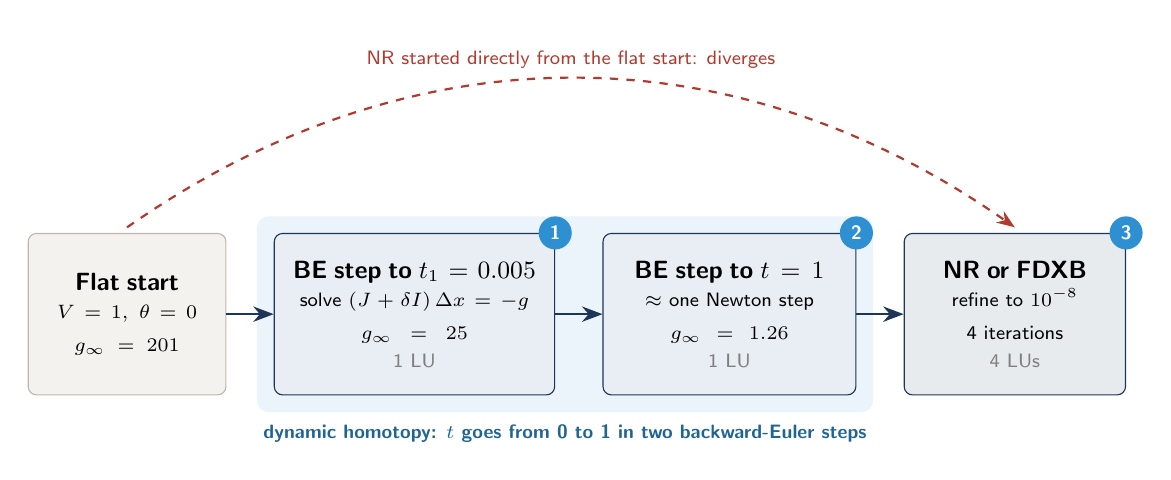
\begin{tikzpicture}[node distance=0.6cm,
  pipe/.style={draw=navy,fill=cloud,rounded corners=3pt,align=center,font=\sffamily\scriptsize,
    text width=#1,minimum height=2.05cm,inner sep=3pt}]
  \node[pipe=2.3cm,fill=mist,draw=rulegrey] (x0) {{\small\textbf{Flat start}}\\[2pt] $V=1,\ \theta=0$\\[4pt] $\ninf{g}=201$};
  \node[pipe=3.35cm,right=of x0] (s1) {{\small\textbf{BE step to $t_1=0.005$}}\\[2pt] solve $(J+\delta I)\,\Delta x=-g$\\[4pt] $\ninf{g}=25$\\[2pt] \textcolor{ink!60}{1 LU}};
  \node[pipe=3.0cm,right=of s1] (s2) {{\small\textbf{BE step to $t=1$}}\\[2pt] $\approx$ one Newton step\\[4pt] $\ninf{g}=1.26$\\[2pt] \textcolor{ink!60}{1 LU}};
  \node[pipe=2.6cm,right=of s2,fill=navy!10,draw=navy] (nr) {{\small\textbf{NR or FDXB}}\\[2pt] refine to $10^{-8}$\\[4pt] 4 iterations\\[2pt] \textcolor{ink!60}{4 LUs}};
  \draw[flow] (x0) -- (s1); \draw[flow] (s1) -- (s2); \draw[flow] (s2) -- (nr);
  \node[badge] at (s1.north east) {1}; \node[badge] at (s2.north east) {2}; \node[badge] at (nr.north east) {3};
  \draw[failred,thick,dashed,-{Stealth}] ([yshift=2pt]x0.north) to[out=35,in=145]
    node[pos=0.5,above,font=\sffamily\scriptsize,text=failred]{NR started directly from the flat start: diverges} ([yshift=2pt]nr.north);
  \begin{scope}[on background layer]
    \node[fill=skyblue!10,rounded corners=4pt,fit=(s1)(s2),inner sep=6pt] (hbox) {};
  \end{scope}
  \node[font=\sffamily\scriptsize\bfseries,text=skyblue!70!black,below=1pt of hbox] {dynamic homotopy: $t$ goes from 0 to 1 in two backward-Euler steps};
\end{tikzpicture}
\caption{The base paper's method at a glance, with the real mismatch norms of one solve of
\code{case109272}. Stage~1 regularises the flat-start Jacobian by $\delta=K/\Delta t_0$; stage~2 is
almost a plain Newton step; stage~3 is ordinary NR from a much better start (\cref{sec:firststep}).}
\Description{Pipeline diagram: flat start, two backward-Euler steps, then Newton-Raphson.}
\label{fig:pipeline}
\end{figure*}

%% ============================================================================ 2 METHODOLOGY
\section{Methodology}\label{sec:methods}

\subsection{The homotopy and its three integrators}
With $\Phi(x,t) = -G_x(x,t)^{-1}G_t(x)$, the three schemes of the paper are
\begin{align}
  \text{FE:}\quad & x_{k+1} = x_k + \Delta t\,\Phi(x_k,t_k), \label{eq:fe}\\
  \text{RK2:}\quad & k_1=\Phi(x_k,t_k),\ \ k_2=\Phi(x_k+\Delta t\,k_1,\,t_{k+1}), \nonumber\\
                   & x_{k+1}=x_k+\tfrac{\Delta t}{2}(k_1+k_2), \label{eq:rk2}\\
  \text{BE:}\quad & x_{k+1} = x_k + \Delta t\,\Phi(x_k,t_{k+1}). \label{eq:be}
\end{align}
The implicit equation of true backward Euler, $x_{k+1}=x_k+\Delta t\,\Phi(x_{k+1},t_{k+1})$, is replaced
by one fixed-point iteration started at $x_k$, as in the paper. What remains ``implicit'' about BE is
only that it evaluates $G_x$ at the \emph{new} time $t_{k+1}$. Every evaluation of $\Phi$ costs one sparse
LU factorization. \Cref{alg:hybrid} gives the complete hybrid method.

\begin{algorithm}[t]
\caption{The base paper's hybrid method}\label{alg:hybrid}
\begin{algorithmic}[1]
\small
\Require $(g,J)$, flat start $\xo$, $K$, times $0=t_0<\dots<t_N=1$, scheme $\in\{\mathrm{FE},\mathrm{RK2},\mathrm{BE}\}$
\State $x \gets \xo$
\For{$k = 0,\dots,N-1$}
  \State $\Delta t \gets t_{k+1}-t_k$; use BE if $k=0$, else the chosen scheme
  \State $x \gets \textsc{Step}(x,t_k,\Delta t)$ \Comment{one LU per $\Phi$}
  \If{a matrix is singular \textbf{or} $\ninf{g(x)}$ is not finite} \State \Return failure \EndIf
\EndFor
\State \Return $\textsc{NR}(x)$ or $\textsc{FDXB}(x)$
\end{algorithmic}
\end{algorithm}

\subsection{What the first step really does}\label{sec:firststep}
At $t_0=0$ the state is $\xo$, so $G_t = g(\xo)$, and the schemes differ only in where they evaluate
$G_x$.

\emph{Forward Euler} uses $G_x(\xo,0)=KI$, in which the network is invisible:
\begin{equation}
  \Delta x_{\mathrm{FE}} = -\frac{\Delta t_0}{K}\,g(\xo) = -50\,g(\xo) \quad(K=10^{-4},\ \Delta t_0=0.005).
\end{equation}
Every unknown is pushed by fifty times its own mismatch, and on the ill-conditioned systems the mismatch
is in the hundreds.

\emph{Backward Euler} uses $G_x(\xo,\Delta t_0) = \Delta t_0 J + (1-\Delta t_0)KI$, so
\begin{equation}
\begin{aligned}
  \Delta x_{\mathrm{BE}} &= -\Delta t_0\bigl[\Delta t_0 J + (1-\Delta t_0)KI\bigr]^{-1} g(\xo)\\
    &= -\bigl[J + \delta' I\bigr]^{-1} g(\xo),\\
  \delta' &= \frac{(1-\Delta t_0)K}{\Delta t_0} \approx \frac{K}{\Delta t_0} = \delta = 0.02 .
\end{aligned}\label{eq:shift}
\end{equation}
This is a Newton step on $g$ with the Jacobian shifted by $\delta I$, structurally a Levenberg--Marquardt
step~\cite{levenberg1944,marquardt1963}. The shift keeps the linear system solvable where the flat-start
Jacobian is nearly singular, and shortens the step in the directions where $J$ is weak, exactly where a
plain Newton step overshoots.

\emph{The last step is almost Newton.} The paper's favourite path has only one more point, $t=1$, where
$G_x = J(x_1)$ and $K$ disappears:
\begin{equation}
\begin{aligned}
  x(1) &= x_1 - (1-\Delta t_0)\,J(x_1)^{-1}\bigl[g(x_1) - K(x_1-\xo)\bigr]\\
       &\approx x_1 - J(x_1)^{-1} g(x_1).
\end{aligned}
\end{equation}
So the two-point BE ``homotopy'' is one shifted Newton step followed by an almost plain Newton step. This
explains why its cost is essentially that of NR, why $\delta$ rather than $K$ or $\Delta t_0$ alone is the
parameter that matters, and why explicit schemes cannot compete with a large final step: at $t=1$ they
would use $G_x$ evaluated at the previous, smaller $t$, still dominated by $KI$ (\cref{fig:firststep-diagram}).

\begin{figure*}[t]
\centering
\begin{tikzpicture}[x=0.27cm,y=0.27cm]
  \begin{scope}
    \node[font=\sffamily\small\bfseries,text=navy,anchor=west] at (0,13.4) {Forward Euler sees $G_x = K I$};
    \draw[rulegrey] (0,0) rectangle (12,12);
    \foreach \i in {0,...,11} \fill[sky!55] (\i+0.1,11.9-\i) rectangle (\i+0.9,11.1-\i);
    \node[font=\sffamily\scriptsize,text=ink!75,align=left,anchor=west] at (12.8,9.6) {only a diagonal of $10^{-4}$:\\ no network information};
    \node[font=\small,anchor=west] at (12.8,5.4) {$\Delta x = -\dfrac{\Delta t_0}{K}\,g(\xo)$};
    \node[font=\sffamily\scriptsize,text=failred,anchor=west] at (12.8,1.6) {$=-50\,g(\xo)$: blows up};
  \end{scope}
  \begin{scope}[xshift=8.4cm]
    \node[font=\sffamily\small\bfseries,text=navy,anchor=west] at (0,13.4) {Backward Euler sees $G_x \propto J + \delta I$};
    \draw[rulegrey] (0,0) rectangle (12,12);
    \foreach \r/\c in {0/3,0/7,1/4,1/9,2/0,2/5,3/1,3/8,4/2,4/6,4/10,5/3,5/11,6/1,6/7,7/4,7/9,8/0,8/5,9/2,9/10,10/6,10/11,11/3,11/8,1/0,3/2,5/4,6/5,8/7,9/8,10/9,11/10,0/1,2/3,4/5,7/8,9/10,10/11}
      \fill[sky!45] (\c+0.15,11.85-\r) rectangle (\c+0.85,11.15-\r);
    \foreach \i in {0,...,11} \fill[navy] (\i+0.1,11.9-\i) rectangle (\i+0.9,11.1-\i);
    \foreach \i in {0,...,11} \draw[skyblue,line width=0.9pt] (\i+0.05,11.95-\i) rectangle (\i+0.95,11.05-\i);
    \node[font=\sffamily\scriptsize,text=ink!75,align=left,anchor=west] at (12.8,9.6) {full network Jacobian,\\ diagonal lifted by $\delta=K/\Delta t_0$};
    \node[font=\small,anchor=west] at (12.8,5.4) {$\Delta x = -\bigl[J+\delta I\bigr]^{-1} g(\xo)$};
    \node[font=\sffamily\scriptsize,text=okgreen,anchor=west] at (12.8,1.6) {a damped Newton step};
  \end{scope}
\end{tikzpicture}
\caption{What each integrator ``sees'' on the first step. Forward Euler inverts $KI$, so its step ignores
the network; backward Euler evaluates $G_x$ one step later, where it is proportional to the real Jacobian
plus a small diagonal shift.}
\Description{Two matrix sketches: a pure diagonal for forward Euler and a sparse network matrix with a lifted diagonal for backward Euler.}
\label{fig:firststep-diagram}
\end{figure*}

\subsection{The refining solvers and the static baseline}
\emph{NR} stops when $\ninf{g}<10^{-8}$ or after 10 iterations (MATPOWER's defaults and the paper's
setting); a singular Jacobian or a non-finite mismatch is a failure. \emph{FDXB} follows MATPOWER's
\code{fdpf}: $B'$ ignores shunts, line charging, taps and resistance, $B''$ keeps the full network without
phase shifters, and both are factorised once. It stops when both the $P$ and the $Q$ mismatch are below
$10^{-8}$, or after 100 $P$--$\theta$ updates. We count $P$ updates plus $Q$ updates, as the paper's
Table~7 does. \emph{GSH-NR}~\cite{freitas2022} is described in the paper only in words, so ours is a
reconstruction: fictitious shunts sized to make the flat start exact at $h=0$ (only the active part at PV
buses, none at the slack bus) and scaled by $(1-h)$, with the resistance and reactance of every branch
connected to the slack bus multiplied by $\delta+(1-\delta)h$. $h$ runs from $\Delta h$ to 1 in steps of
$\Delta h$, every point is a full NR solve (tolerance $10^{-8}$, at most 10 iterations), and the reported
count is the total number of NR iterations over all points. The pair $(\Delta h,\delta)$ is taken per
system from the paper's Table~7 (\cref{tab:params}).

\subsection{Modifications to the method}\label{sec:mods}
Every modification is a switch on top of the untouched reproduction. Building the reproduction first
showed (\cref{sec:firststep}) that the method is a shifted Newton step followed by a near-Newton step, so
the Newton stages became the most promising place to intervene. \Cref{fig:switches} shows where each switch
acts.

\paragraph{M1: optimal multiplier in NR}
Iwamoto and Tamura~\cite{iwamoto1981} scale each Newton step $\Delta x$ by $\mu$. With $a=g(x)$ and
$c=g(x+\Delta x)$, the mismatch along the step is modelled as $g(x+\mu\Delta x)\approx(1-\mu)a+\mu^2c$,
exact when $g$ is quadratic (rectangular coordinates). Minimising $\norm{(1-\mu)a+\mu^2c}_2^2$ gives the cubic
\begin{equation}
  2(c^{\top}c)\,\mu^3 - 3(a^{\top}c)\,\mu^2 + (a^{\top}a + 2a^{\top}c)\,\mu - a^{\top}a = 0,
\end{equation}
of which we take the real root in $(0,2]$ with the smallest model mismatch. It costs no extra LU, and near
the solution $\mu\to1$, so quadratic convergence is kept.

\paragraph{M2: Newton corrector after every step}
As in predictor--corrector continuation~\cite{allgower2003}, after any step to $t_{k+1}$ we take one Newton
step on $G(x,t_{k+1})=0$: $x_{k+1}\gets x_{k+1}-G_x(x_{k+1},t_{k+1})^{-1}G(x_{k+1},t_{k+1})$, at one extra LU
per path point. The corrector is applied after every step, the first BE step included. At $t=1$ it is
exactly one NR step on $g$.

\paragraph{M3: Richardson error control of the path steps}
After the BE step to $t_1=\Delta t_0$, each attempt from $t$ with step $\Delta t$ computes one full step
$x_{\mathrm{full}}$ and two half steps $x_{\mathrm{half}}$ (step doubling~\cite{hairer1993}). For a rule of
order $p$,
\begin{gather}
  \varepsilon = \frac{\ninf{x_{\mathrm{half}}-x_{\mathrm{full}}}}{2^p-1}, \qquad
  x_{\mathrm{new}} = x_{\mathrm{half}} + \frac{x_{\mathrm{half}}-x_{\mathrm{full}}}{2^p-1}, \\
  \Delta t \gets \Delta t\cdot\min\!\Bigl(4,\ \max\bigl(0.1,\ 0.9\,(\mathrm{tol}/\varepsilon)^{1/(p+1)}\bigr)\Bigr).
\end{gather}
The step is accepted if $\varepsilon\le\mathrm{tol}=0.5$ (radians and per unit), and the extrapolated
$x_{\mathrm{new}}$ is kept; if $g(x_{\mathrm{new}})$ is not finite, the two-half-step result is kept
instead. A step that breaks down (singular matrix or non-finite mismatch) is retried at a quarter of its
size, and a path that needs more than 150 LUs is stopped and counted as a failure (\cref{alg:richardson}).
Every attempt costs three steps. The step rule can be BE ($p=1$), FE ($p=1$), RK2 ($p=2$) or RK4 ($p=4$);
the first step to $t_1$ is always BE. The large tolerance is deliberate: the path only has to end inside
NR's region of convergence.

\begin{algorithm}[t]
\caption{Richardson-controlled path}\label{alg:richardson}
\begin{algorithmic}[1]
\small
\State $x\gets\textsc{BE}(\xo,0,\Delta t_0)$;\ $t\gets\Delta t_0$;\ $\Delta t\gets 1-\Delta t_0$
\While{$t<1$ \textbf{and} at most 150 LUs used}
  \State $\Delta t\gets\min(\Delta t,1-t)$;\ $x_f\gets\textsc{Step}(x,t,\Delta t)$
  \State $x_h\gets\textsc{Step}(\textsc{Step}(x,t,\tfrac{\Delta t}{2}),t+\tfrac{\Delta t}{2},\tfrac{\Delta t}{2})$
  \If{a step broke down} $\Delta t\gets\Delta t/4$; \textbf{continue} \EndIf
  \State $\varepsilon\gets\ninf{x_h-x_f}/(2^p-1)$
  \If{$\varepsilon\le\mathrm{tol}$} $x\gets x_h+(x_h-x_f)/(2^p-1)$; $t\gets t+\Delta t$ \EndIf
  \State $\Delta t\gets\Delta t\cdot\min(4,\max(0.1,\,0.9(\mathrm{tol}/\varepsilon)^{1/(p+1)}))$
\EndWhile
\end{algorithmic}
\end{algorithm}

\paragraph{M4: adaptive time points by mismatch}
A cheaper rule keeps the first step to $t_1$, then tries to jump straight to $t=1$. A step is kept if it
reduced $\ninf{g}$ and otherwise halved (at most six times); after an accepted step the next one is
doubled. Rejected trials still count as LUs.

\paragraph{M5--M8: four further ideas}
\textbf{M5, BE-chord:} three fixed-point iterations
$\hat x\gets x_k-\Delta t\,G_x(x_k,t_{k+1})^{-1}G_t(\hat x)$, started at $\hat x=x_k$ and reusing one LU. The
paper writes BE as the fixed-point iteration of its eq.~(19) and uses one iteration; M5 tests whether more
iterations help. It replaces BE on every step, the first included. \textbf{M6, RK4}
(classical fourth order, four LUs per step) with fixed steps after a BE first step (the paper's future
work). \textbf{M7, scaled homotopy:} $K D(x-\xo)$ with $D=|\mathrm{diag}\,J(\xo)|$ normalised to mean one
(zero diagonal entries replaced by the smallest nonzero one), in the spirit of~\cite{freitas2023}.
\textbf{M8, Newton homotopy:} $G(x,t)=g(x)-(1-t)g(\xo)$~\cite{watson1989}, which has $G_x=J(x)$ and no $KI$
term. M7 and M8 are followed with BE.

\begin{figure*}[t]
\centering
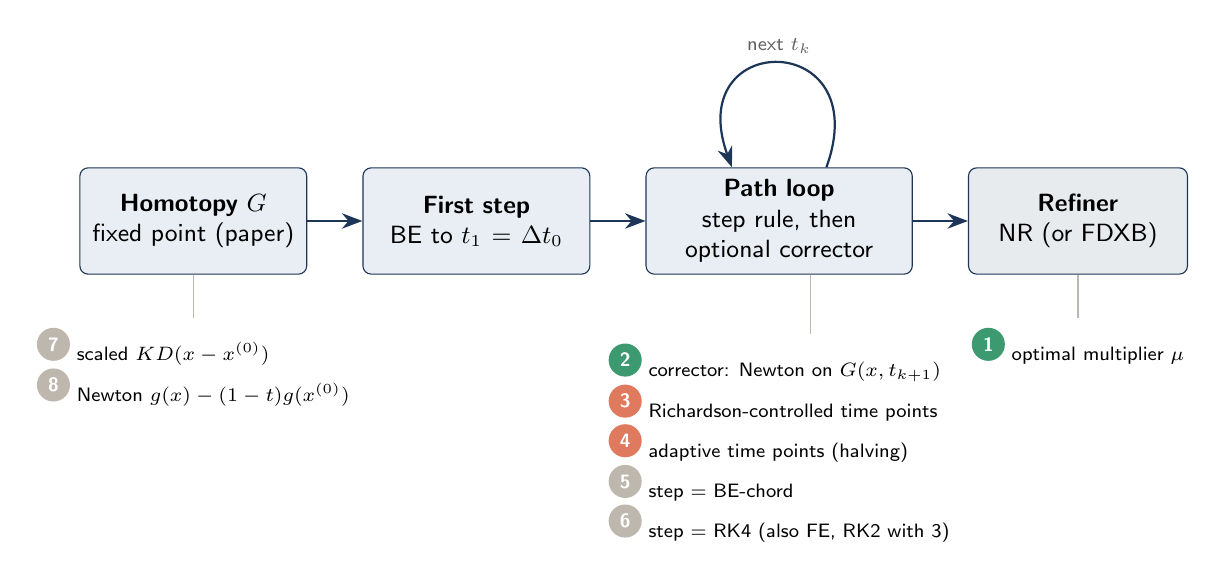
\begin{tikzpicture}[node distance=0.7cm]
  \node[stage=2.6cm] (g) {\textbf{Homotopy $G$}\\ fixed point (paper)};
  \node[stage=2.6cm,right=of g] (f) {\textbf{First step}\\ BE to $t_1=\Delta t_0$};
  \node[stage=3.1cm,right=of f] (l) {\textbf{Path loop}\\ step rule, then\\ optional corrector};
  \node[stage=2.5cm,right=of l,fill=navy!10,draw=navy] (r) {\textbf{Refiner}\\ NR (or FDXB)};
  \draw[flow] (g) -- (f); \draw[flow] (f) -- (l); \draw[flow] (l) -- (r);
  \draw[flow] ([xshift=6mm]l.north) to[out=70,in=110,looseness=4] node[above,note]{next $t_k$} ([xshift=-6mm]l.north);
  \node[font=\sffamily\scriptsize,align=left,anchor=north] (tg) at ([yshift=-0.55cm]g.south) {\tikz\node[xbadge]{7}; scaled $K D(x-\xo)$\\ \tikz\node[xbadge]{8}; Newton $g(x)-(1-t)g(\xo)$};
  \node[font=\sffamily\scriptsize,align=left,anchor=north] (tl) at ([yshift=-0.75cm]l.south) {\tikz\node[gbadge]{2}; corrector: Newton on $G(x,t_{k+1})$\\ \tikz\node[badge,fill=coral]{3}; Richardson-controlled time points\\ \tikz\node[badge,fill=coral]{4}; adaptive time points (halving)\\ \tikz\node[xbadge]{5}; step = BE-chord\\ \tikz\node[xbadge]{6}; step = RK4 (also FE, RK2 with 3)};
  \node[font=\sffamily\scriptsize,align=left,anchor=north] (tr) at ([yshift=-0.55cm]r.south) {\tikz\node[gbadge]{1}; optimal multiplier $\mu$};
  \draw[rulegrey] (g.south) -- (tg.north); \draw[rulegrey] (l.south) ++(0.4,0) -- ([xshift=0.4cm]tl.north); \draw[rulegrey] (r.south) -- (tr.north);
\end{tikzpicture}
\caption{Where each of the eight modifications acts. Green: the two that help on their own and together;
orange: the two path-control rules, which help on some systems at a price; grey: the four that did not work
(\cref{sec:modresults}).}
\Description{Pipeline of homotopy, first step, path loop and refiner with numbered modification badges.}
\label{fig:switches}
\end{figure*}

\subsection{Numerical studies from our proposal}\label{sec:studiesmethod}
\paragraph{Spectrum of the flat-start Jacobian}
The first BE step solves with $J+\delta I$, whose eigenvalues are those of $J$ moved by $\delta$. The
largest eigenvalue modulus comes from the power method~\cite{golub2013}; because $J$ is non-symmetric and
its dominant eigenvalues may form a complex or $\pm\lambda$ pair, we iterate with $J$ applied twice and take
$\sqrt{\norm{J^2x}/\norm{x}}$. The smallest modulus comes from shifted inverse iteration: the power method on
$(J-\sigma I)^{-1}$ using one sparse LU of $J-\sigma I$, with $\sigma=0$ for $J$ and $\sigma=-\delta$ for
$J+\delta I$. ARPACK~\cite{arpack} (via SciPy) is an independent check.

\paragraph{Feasibility maps} The paper's method (BE on $\{0,\Delta t_0,1\}$, then NR) is run on an
$8\times11$ grid, $\Delta t_0\in[0.001,0.2]$ and $K\in[10^{-6},10^{-1}]$, recording whether each run reaches
the reference solution, another root, or fails.

\paragraph{Golden-section tuning of $\delta$} The objective is the total LU count (a failure costs 50)
plus a tie-break $0.1\log_{10}\ninf{g(x(1))}$. Golden-section search~\cite{kiefer1953} runs over
$\log_{10}\delta\in[-4,1]$ at $\Delta t_0=0.005$, then over $\log_{10}\Delta t_0\in[-3,-0.5]$, each to a
bracket of 0.05 decades (21 solves per system). Since the objective is piecewise constant and not unimodal,
the best point seen is returned.

\paragraph{Linear solvers from scratch} Gauss elimination with partial pivoting and back substitution,
and Doolittle LU with partial pivoting ($PA=LU$, $L$ and $U$ in one array, permutation as an index vector)
with forward and back substitution. Both are dense and $\mathcal{O}(n^3)$; the paper's BE path, NR and FDXB
are repeated with every linear system solved this way.

%% ============================================================================ 3 IMPLEMENTATION
\section{Implementation and Experiments}\label{sec:impl}

\subsection{Software architecture}
Everything in \code{dynhomotopy} is written against one interface: a problem supplies $g(x)$ and $J(x)$,
nothing else, so the paper's $2\times2$ tutorial problem and the 109{,}272-bus grid go through the same
solver and integrator code (\cref{fig:arch}). The power flow \emph{model}---reading a MATPOWER case,
renumbering buses, building $Y_{\mathrm{bus}}$, $S_{\mathrm{bus}}$, $B'$, $B''$ and the derivatives
$\partial S/\partial V$ for the Jacobian---uses PYPOWER~\cite{pypower}, a Python port of
MATPOWER~\cite{matpower}, which contains only formulas, no solving. Every numerical method (NR, FDXB,
GSH-NR, the homotopy, the integrators, the LU counter and everything in \code{improvements}) is our own code,
built on NumPy~\cite{numpy} and SciPy~\cite{scipy}. Sparse linear systems are solved with SuperLU~\cite{superlu}
through SciPy, and every factorization in the program goes through one counter, which is how cost is
measured. Figures are drawn with Matplotlib~\cite{matplotlib}. The modifications live in a second package
that imports the first and never edits it; a test asserts that with every switch off the modified solver
returns the paper's method bit for bit. \Cref{lst:core} shows the core of the method.

\begin{figure*}[t]
\centering
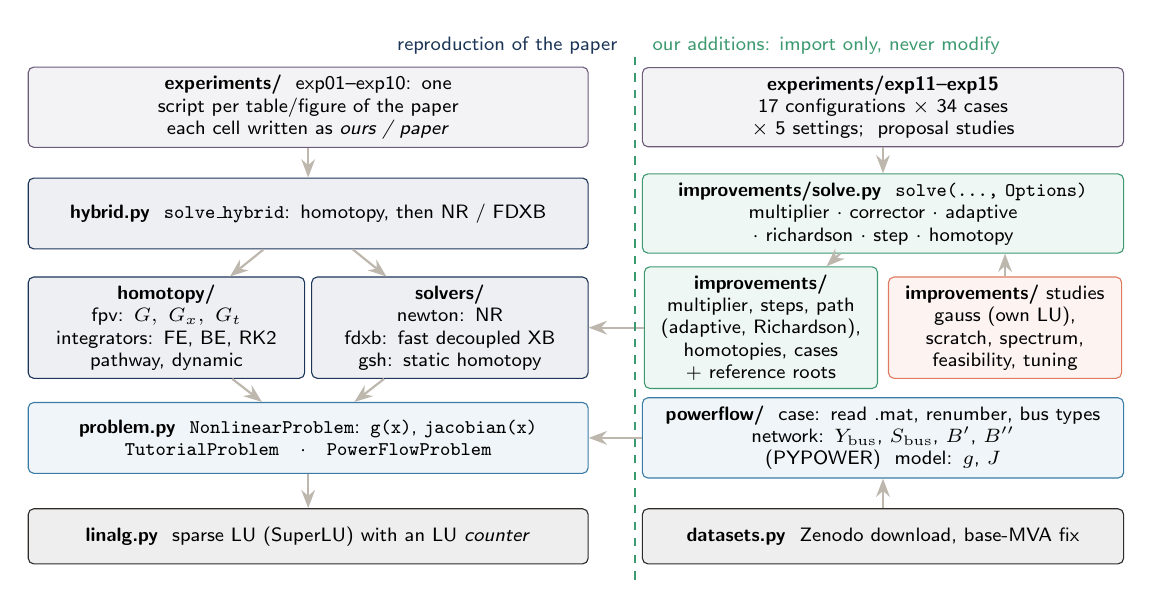
\begin{tikzpicture}[
  box/.style={draw=#1,fill=#1!8,rounded corners=2pt,font=\sffamily\scriptsize,align=center,inner sep=3pt,minimum height=0.9cm},
  x=1cm,y=1cm]
  \node[box=plum,text width=6.9cm] (exp) at (3.6,4.2) {\textbf{experiments/}\ \ exp01--exp10: one script per table/figure of the paper\\ each cell written as \emph{ours / paper}};
  \node[box=plum,text width=5.9cm] (exp11) at (10.9,4.2) {\textbf{experiments/exp11--exp15}\\ 17 configurations $\times$ 34 cases $\times$ 5 settings;\ \ proposal studies};
  \node[box=navy,text width=6.9cm] (hyb) at (3.6,2.85) {\textbf{hybrid.py}\ \ \code{solve\_hybrid}: homotopy, then NR / FDXB};
  \node[box=sage,text width=5.9cm] (imp) at (10.9,2.85) {\textbf{improvements/solve.py}\ \ \code{solve(..., Options)}\\ multiplier $\cdot$ corrector $\cdot$ adaptive $\cdot$ richardson $\cdot$ step $\cdot$ homotopy};
  \node[box=navy,text width=3.3cm] (hom) at (1.8,1.4) {\textbf{homotopy/}\\ fpv: $G,\ G_x,\ G_t$\\ integrators: FE, BE, RK2\\ pathway, dynamic};
  \node[box=navy,text width=3.3cm] (sol) at (5.4,1.4) {\textbf{solvers/}\\ newton: NR\\ fdxb: fast decoupled XB\\ gsh: static homotopy};
  \node[box=sage,text width=2.75cm] (impm) at (9.35,1.4) {\textbf{improvements/}\\ multiplier, steps, path (adaptive, Richardson), homotopies, cases + reference roots};
  \node[box=coral,text width=2.75cm] (ext) at (12.45,1.4) {\textbf{improvements/} studies\\ gauss (own LU), scratch, spectrum, feasibility, tuning};
  \node[box=sky,text width=6.9cm] (prob) at (3.6,0.0) {\textbf{problem.py}\ \ \code{NonlinearProblem}: \code{g(x)}, \code{jacobian(x)}\\ \code{TutorialProblem}\quad$\cdot$\quad \code{PowerFlowProblem}};
  \node[box=sky,text width=5.9cm] (pf) at (10.9,0.0) {\textbf{powerflow/}\ \ case: read .mat, renumber, bus types\\ network: $Y_{\mathrm{bus}}$, $S_{\mathrm{bus}}$, $B'$, $B''$ (PYPOWER)\ \ model: $g$, $J$};
  \node[box=ink,text width=6.9cm,minimum height=0.7cm] (lin) at (3.6,-1.25) {\textbf{linalg.py}\ \ sparse LU (SuperLU) with an LU \emph{counter}};
  \node[box=ink,text width=5.9cm,minimum height=0.7cm] (ds) at (10.9,-1.25) {\textbf{datasets.py}\ \ Zenodo download, base-MVA fix};
  \foreach \a/\b in {exp/hyb,exp11/imp,hyb/hom,hyb/sol,imp/impm,hom/prob,sol/prob,prob/lin}
    \draw[-{Stealth},rulegrey,thick] (\a) -- (\b);
  \draw[-{Stealth},rulegrey,thick] (impm.west) -- (sol.east);
  \draw[-{Stealth},rulegrey,thick] (ext.north) -- (ext.north |- imp.south);
  \draw[-{Stealth},rulegrey,thick] (pf.west) -- (prob.east);
  \draw[-{Stealth},rulegrey,thick] (ds.north) -- (pf.south);
  \draw[sage,thick,dashed] (7.75,-1.8) -- (7.75,4.85);
  \node[font=\sffamily\scriptsize,text=sage,anchor=south west] at (7.85,4.75) {our additions: import only, never modify};
  \node[font=\sffamily\scriptsize,text=navy,anchor=south east] at (7.65,4.75) {reproduction of the paper};
\end{tikzpicture}
\caption{Architecture of the implementation. Every solver sees only $g(x)$ and $J(x)$, and every LU
factorization in the program goes through one counter.}
\Description{Layered architecture diagram of the dynhomotopy and improvements packages.}
\label{fig:arch}
\end{figure*}

\begin{lstlisting}[style=py,caption={The core of the method (\texttt{homotopy/fpv.py}, \texttt{homotopy/integrators.py}), lightly trimmed.},label=lst:core,float=t]
class FixedPointHomotopy:       # G = t g(x) + (1-t) K (x - x0)
    def G(self, x, t):
        return t*self.problem.g(x) + (1-t)*self.K*(x - self.x0)
    def Gx(self, x, t):
        return (t*self.problem.jacobian(x)
                + (1-t)*self.K*self.eye).tocsc()
    def Gt(self, x):
        return self.problem.g(x) - self.K*(x - self.x0)
    def dxdt(self, x, t):       # one sparse LU per call, counted
        return -solve(self.Gx(x, t), self.Gt(x), self.counter)

def forward_euler(h, x, t, dt):  return x + dt*h.dxdt(x, t)
def backward_euler(h, x, t, dt): return x + dt*h.dxdt(x, t+dt)
def runge_kutta2(h, x, t, dt):
    k1 = h.dxdt(x, t); k2 = h.dxdt(x + dt*k1, t + dt)
    return x + dt/2*(k1 + k2)
\end{lstlisting}

\subsection{Datasets and benchmarks}\label{sec:data}
All systems are MATPOWER cases from two public Zenodo records by Tostado-V\'eliz, Kamel and Jurado, the
same files the paper uses: record 3514739 holds the \emph{ill-conditioned} systems~\cite{tostado2019ill},
built by gluing copies of European PEGASE~\cite{pegase} and Polish networks together, and record 3491654
the \emph{loading-limit} systems~\cite{tostado2019limit}, in which every load of a standard case was scaled
up until NR from a flat start was about to stop converging. The code downloads each file on first use.
The paper uses nine of these systems; for the modification study we added every other system in the two
records that loads, giving 34 (\cref{tab:systems,fig:systems}). Twenty-five of them were never seen while
the paper's parameters were chosen, so they test whether those parameters generalise. The replicated
construction is visible in the Jacobian (\cref{fig:spy}, \cref{app:extra}): \code{case54636} and \code{case109272}, four and
eight copies of the same network, behave \emph{identically} in every experiment, which is a useful check on
the paper (\cref{sec:audit}). Throughout the report \code{case500limit} and \code{case2000limit} are short
for the files \code{case\_ACTIVSg500limit} and \code{case\_ACTIVSg2000limit}; the paper uses both forms.

\begin{table*}[t]
\centering
\caption{The 34 test systems. $n$ is the number of unknowns, nnz the nonzeros of the Jacobian at the flat
start, and the last column the NR iterations needed from the flat start (limit 10).}
\label{tab:systems}
\footnotesize
\setlength{\tabcolsep}{5pt}
\begin{tabular}{@{}l l r r r r r r@{}}
\toprule
\thead{Case} & \thead{Built from} & \thead{Buses} & \thead{PV} & \thead{$n$} & \thead{nnz($J$)} & \thead{$\ninf{g(\xo)}$} & \thead{NR flat} \\
\midrule
\rows{generated/systems_rows.tex}
\bottomrule
\end{tabular}
\end{table*}

\begin{figure*}[t]
\centering
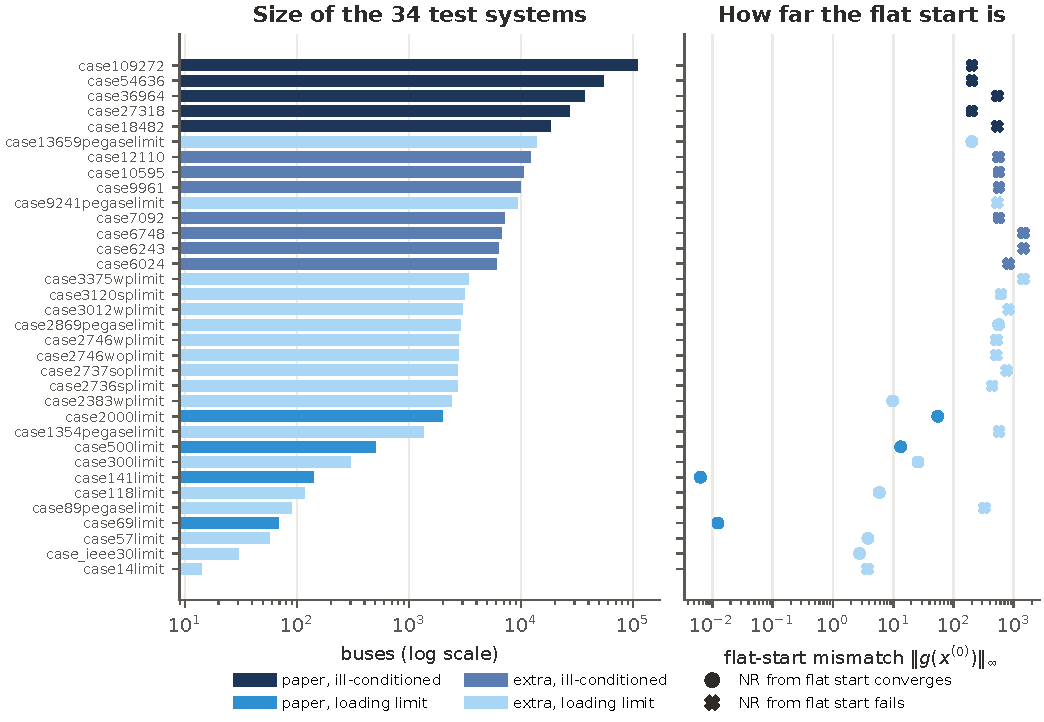
\includegraphics[width=0.92\textwidth]{figures/systems.pdf}
\caption{Size and flat-start mismatch of all 34 systems. Size alone does not decide difficulty: NR from the
flat start fails on the 14-bus limit case and succeeds on the 13{,}659-bus one. The failing systems share a
large initial mismatch.}
\Description{Bar chart of system size and flat-start mismatch.}
\label{fig:systems}
\end{figure*}

\paragraph{Four details that change numbers}
(i)~\code{case69limit} and \code{case141limit} are stored with $\text{baseMVA}=10$, but the paper's Tables
2--5 come out only on \SI{100}{MVA}, so we use 100 (\cref{sec:audit}). (ii)~The flat start includes the
slack angle; for NR-MAT (NR from the stored operating point) we shift the stored angles so the slack is at
zero. (iii)~Six of the 22 limit cases converge from the flat start in \emph{exactly} ten NR iterations and
eleven more fail at ten, so any change worth one NR iteration can flip a limit case. (iv)~The power flow
equations have several roots, and a mismatch below $10^{-8}$ does not say which one was found. For every
system the \emph{reference} solution is the one NR reaches from the initial guess stored in the case file
(up to 50 iterations, with the optimal multiplier as a fallback); a run is \emph{solved} only if every bus
voltage is within \SI{e-4}{pu} of it.

\subsection{Experimental setup and parameter choices}
\paragraph{Reproduction} Each result of the paper has its own script (exp01--exp10,
\cref{tab:scripts}). Unless stated otherwise $K=10^{-4}$ and $\Delta t_0=0.005$ ($\delta=0.02$), NR
tolerance $10^{-8}$ with 10 iterations, and the paths are those of the paper: $\{0,0.005,0.01,0.51,1\}$ for
Tables 2--4, $\{0,0.005,0.01,0.02,0.12,0.62,1\}$ for Table~5, $\{0,0.05,0.1,t_3,1\}$ with $K=10^{-3}$ for
Figure~3 and Table~6, and $\{0,0.005,1\}$ for BE in Table~7. Timings are medians of seven repetitions.

\paragraph{Modification study} Every configuration runs on all 34 systems under five settings of
$(\Delta t_0,K)$, all on the path $\{0,\Delta t_0,1\}$: S1 $(0.005,10^{-4})$ the paper's setting,
S2 $(0.05,10^{-3})$ and S3 $(0.1,2\times10^{-3})$ from the paper's Section 4.4, S4 $(0.005,10^{-5})$ a weak
$K$, and S5 $(0.005,10^{-3})$ a strong $K$. M1, M2 and M4 run in all eight on/off combinations; M3 with each
of BE, FE, RK2 and RK4 and together with M1; and M5--M8 alone: 17 configurations, 2{,}890 runs. Cost is the
number of LU factorizations, which does not depend on the machine. If a configuration solves a run the
paper's method does not, the paper's method is re-run with 30 NR iterations to classify the gain as a
\emph{speed-up} (it then reaches the reference), a \emph{root fix} (it reaches another root) or a
\emph{rescue} (it still diverges).

\paragraph{Parameter summary} \Cref{tab:params} lists every parameter of the methods and studies, with
the value used and where it comes from. All values are read from the code.

\begin{table*}[t]
\centering
\caption{Parameters of the methods, modifications and studies, as set in the code.}
\label{tab:params}
\footnotesize
\begin{tabularx}{\textwidth}{@{}>{\raggedright\arraybackslash}p{4.2cm} >{\raggedright\arraybackslash}X >{\raggedright\arraybackslash}p{4.2cm}@{}}
\toprule
\thead{Parameter} & \thead{Value} & \thead{Source} \\
\midrule
Homotopy factor $K$, first step $\Delta t_0$ & $10^{-4}$, 0.005 ($\delta=K/\Delta t_0=0.02$); $10^{-3}$ with $\Delta t_0=0.05$ and $2\times10^{-3}$ with $\Delta t_0=0.1$ in Section~4.4, Figure~3 and Table~6 & base paper \\
NR & tolerance $\ninf{g}<10^{-8}$, at most 10 iterations (30 to classify gains, 50 for the reference solution) & paper / MATPOWER defaults \\
FDXB & tolerance $10^{-8}$ on $P$ and $Q$ mismatch, at most 100 $P$--$\theta$ updates & MATPOWER \code{fdpf} \\
GSH-NR $(\Delta h,\delta)$ & \code{case18482} (0.5, 1); \code{case27318} (0.25, 0.125); \code{case36964} (0.25, 1); \code{case54636}, \code{case109272} (0.01, 0.01); the four limit cases (1, 1) & paper, Table~7 \\
Tutorial & $\xo=(1,1)$, $\Delta t_0=0.01$, then constant $\Delta t\in\{0.5,0.125\}$, $K\in\{0.05,0.01,0.005\}$, NR tolerance $10^{-5}$ & paper, Section~3.3 \\
Paths for Tables 7 and 8 & BE: $\{0,0.005,1\}$; RK2: $\{0,0.005,0.01,0.02,0.12,0.42,0.72,1\}$ & paper \\
Reference solution & NR from the stored initial guess, up to 50 iterations, optimal multiplier as fallback; a run is on the reference if $\max_k|V_k-V_k^{\mathrm{ref}}|<10^{-4}$\,pu & ours \\
Richardson control (M3) & tol $=0.5$, step factor $\min(4,\max(0.1,0.9(\mathrm{tol}/\varepsilon)^{1/(p+1)}))$, retry at $\Delta t/4$ after a breakdown, at most 150 LUs per path & ours \\
Adaptive steps (M4) & at most 6 halvings per step, next step doubled after an accepted one & ours \\
BE-chord (M5) & 3 fixed-point iterations per step with one LU & ours \\
Optimal multiplier (M1) & real root of the cubic in $(0,2]$ with the smallest model mismatch, else $\mu=1$ & Iwamoto and Tamura \\
Power method / inverse iteration & random start (seed 0), relative tolerance $10^{-6}$, at most 500 / 200 iterations; shift $\sigma=-0.02$ for $J+\delta I$ & ours \\
Feasibility grid & $\Delta t_0\in\{0.001,0.0025,0.005,0.01,0.025,0.05,0.1,0.2\}$, 11 values of $K$ log-spaced in $[10^{-6},10^{-1}]$, path $\{0,\Delta t_0,1\}$; systems \code{case18482}, \code{case36964}, \code{case6024}, \code{case2000limit} & ours \\
Golden-section tuning & $\log_{10}\delta\in[-4,1]$ at $\Delta t_0=0.005$, then $\log_{10}\Delta t_0\in[-3,-0.5]$; bracket 0.05, at most 25 evaluations per search; failure costs 50 LUs; tie-break $0.1\log_{10}\ninf{g(x(1))}$ & ours \\
\bottomrule
\end{tabularx}
\end{table*}

\paragraph{Verification and software} Before any comparison, the building blocks are checked by 24
automated tests (pytest~\cite{pytest}), all of which pass on the current code: the analytic Jacobian
against finite differences on \code{case69limit} and \code{case500limit}; the path generator against the
paper's time grids; the BE first step against the paper's linearised static homotopy (eqs.~25 and 27, to
$10^{-10}$); NR on the tutorial in exactly the paper's 11 iterations; the NR-MAT and NR-flat counts, a full
row of Table~4 and the FDXB count of Table~7 for \code{case2000limit}; the switch-off identity; the optimal
multiplier, the corrector, the adaptive rule, the explicit rules' BE first step and both alternative
homotopies; our Gauss elimination and LU against NumPy, with pivoting past a zero diagonal, and with the
same Newton iterates as SuperLU on \code{case500limit}; the eigenvalue routines on a diagonal matrix;
golden-section search on a parabola; Richardson control reaching $t=1$; and both command-line tools. The
software dependencies are those of the repository's \code{requirements.txt}: NumPy~$\ge$1.24,
SciPy~$\ge$1.10, Matplotlib~$\ge$3.7, PYPOWER~$\ge$5.1 and pytest~$\ge$7.

%% ============================================================================ 4 RESULTS
\section{Results and Discussion}\label{sec:results}

\subsection{Reproducing the base paper}\label{sec:repro}

\paragraph{The two-variable tutorial} The paper first tests the idea on $g_1=x_1^2+x_2^2-2x_1x_2-1$,
$g_2=x_1+x_2-2$ from $\xo=(1,1)$, where the Jacobian is singular. The system has two roots, $A=(1.5,0.5)$
and $B=(0.5,1.5)$, and the singular set is the line $x_1=x_2$ through the start. \Cref{fig:tutorial} draws
what the integrators do in this plane, which the paper shows only as mismatch curves: with $K=0.05$ all
three stay near the exact path; with $K=0.005$ the explicit ones overshoot across the singular line and NR
then converges to root $B$, while BE reaches $A$. \Cref{tab:tutorial} and \cref{fig:tut-repro} (\cref{app:extra}) compare
iteration counts: NR alone matches the paper for $\epsilon=0.005$ and $0.01$; BE is the best start for NR in
every hybrid panel, as in the paper, though some counts differ by one or two.

\begin{figure*}[t]
\centering
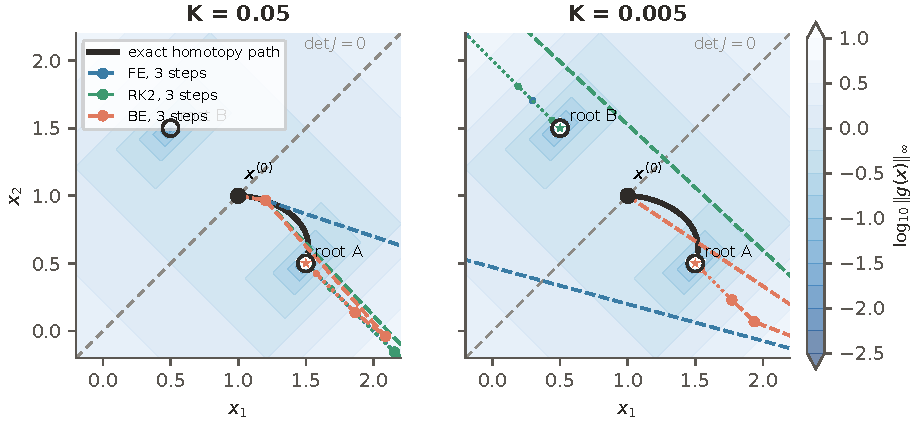
\includegraphics[width=0.9\textwidth]{figures/tutorial_geometry.pdf}
\caption{The tutorial in the $(x_1,x_2)$ plane, $\Delta t_0=0.01$ then $\Delta t=0.5$. Background:
$\log_{10}\ninf{g}$. Black: the exact homotopy path; dashed: the three coarse integrations; dotted: the NR
iterations; stars: where NR ends. At the smaller $K$ the explicit schemes cross $\det J=0$ and NR finds the
other root.}
\Description{Contour plots of the tutorial problem with integration paths.}
\label{fig:tutorial}
\end{figure*}

\begin{table}[t]
\centering
\caption{Tutorial: NR iterations to $\ninf{g}<10^{-5}$, ours and read off the paper's plots, and the root
reached.}
\label{tab:tutorial}
\footnotesize
\setlength{\tabcolsep}{3pt}
\begin{tabular}{@{}l c c c c c@{}}
\toprule
\thead{Run} & \thead{$\Delta t$} & \thead{$K$} & \thead{Ours} & \thead{Paper} & \thead{Root} \\
\midrule
NR, $\epsilon=0.005$ & -- & -- & 11 & 11 & $A$ \\
NR, $\epsilon=0.01$ & -- & -- & 10 & 10 & $A$ \\
NR, $\epsilon=0.05$ & -- & -- & 8 & 9 & $A$ \\
\midrule
FE/BE/RK2 & 0.5 & 0.05 & 6/4/4 & 6/3/6 & $A$/$A$/$A$ \\
FE/BE/RK2 & 0.5 & 0.01 & 6/2/4 & 4/2/4 & $B$/$A$/$B$ \\
FE/BE/RK2 & 0.5 & 0.005 & 8/4/7 & 6/3/7 & $B$/$A$/$B$ \\
FE/BE/RK2 & 0.125 & 0.05 & 3/3/2 & 3/2/3 & $A$/$A$/$A$ \\
\bottomrule
\end{tabular}
\end{table}

\paragraph{The first time step} \Cref{fig:first} measures the paper's Section~4.2.1 on all nine systems:
with $K=10^{-4}$, FE multiplies the mismatch by factors between $7\times10^{3}$ (\code{case69limit}) and
$1.8\times10^{10}$ (\code{case18482}), and RK2, which evaluates its second slope at the FE point, by factors
between $1.9\times10^{3}$ and $1.4\times10^{10}$. BE reduces the mismatch by about a factor of eight on every
ill-conditioned system (533 to 65 or 66, 201 to 25), the values the paper prints in the $t=0.005$ column of
its Table~4, and it also reduces it on all four limit cases. Taking the FE step with $K=1$, the value earlier
work used, makes the blow-up much smaller but does not remove it: the mismatch still grows on all nine
systems, for example from 533 to $1.3\times10^{5}$ on \code{case18482} and from 55 to 631 on
\code{case2000limit}.

\begin{figure}[t]
\centering
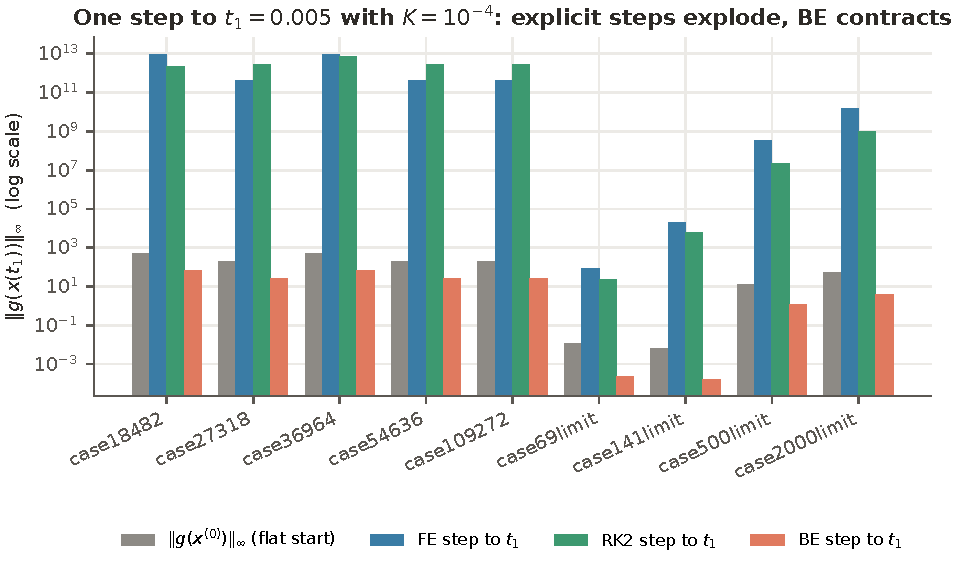
\includegraphics[width=\columnwidth]{figures/first_step.pdf}
\caption{Mismatch after the single first step to $t_1=0.005$, $K=10^{-4}$ (log scale). Grey is the flat
start. FE and RK2 make every system worse by orders of magnitude; BE improves every one.}
\Description{Grouped bar chart of mismatch after the first step.}
\label{fig:first}
\end{figure}

\paragraph{Tables 2--5: mismatch along the path} On the paper's path $\{0, 0.005, 0.01, 0.51, 1\}$ our BE results
(\cref{tab:be}) match the paper almost digit for digit, including the three NR iterations that follow; the
FE and RK2 tables (\cref{tab:fe,tab:rk2}, \cref{app:tables}) match wherever the schemes stay finite and blow up
at the same point where they diverge. With the growing steps of Table~5 (\cref{tab:t5}, \cref{app:extra}) all three schemes
give NR a usable start. \Cref{fig:fidelity} puts all 255 numeric cells of Tables 2--5 on one plot: 246
(96\%) agree within a factor of two and 200 (78\%) within 10\%, the rounding of the paper's two printed
digits. Of the nine outliers, seven are divergent FE/RK2 values above $10^{3}$, one is a Table~2 cell
discussed in \cref{sec:audit}, and one is a final NR mismatch near $10^{-11}$.

\begin{table*}[t]
\centering
\caption{Table 4 re-run: $\ninf{g}$ along the BE path $\{0,0.005,0.01,0.51,1\}$ and after each of the first
three NR iterations, $K=10^{-4}$. Each case shows our value above the paper's.}
\label{tab:be}
\scriptsize
\setlength{\tabcolsep}{4pt}
\begin{tabular}{@{}l l r r r r r r r r l@{}}
\toprule
\thead{Case} & & \thead{$t{=}0$} & \thead{0.005} & \thead{0.01} & \thead{0.51} & \thead{1} & \thead{NR 1} & \thead{NR 2} & \thead{NR 3} & \thead{Result} \\
\midrule
\rows{generated/table4_rows.tex}
\bottomrule
\end{tabular}
\end{table*}

\begin{figure}[t]
\centering
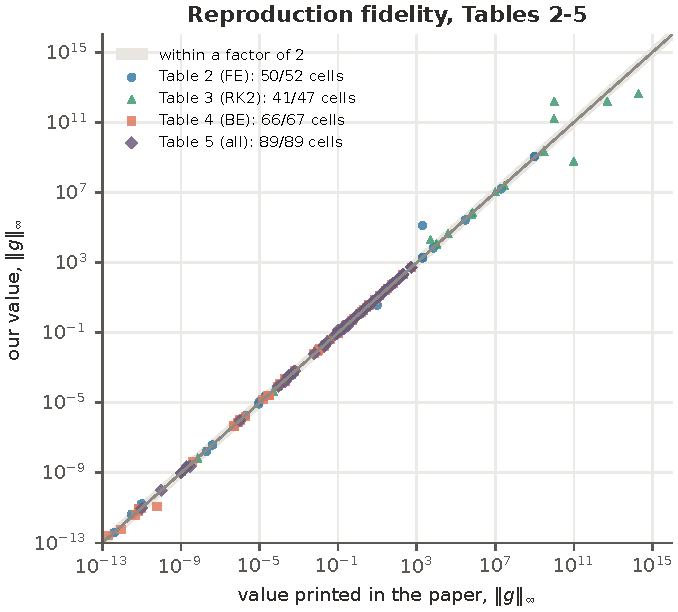
\includegraphics[width=0.9\columnwidth]{figures/fidelity.pdf}
\caption{Every numeric cell of the paper's Tables 2--5 against our value, on log axes spanning 28 orders of
magnitude. The grey band is agreement within a factor of two.}
\Description{Scatter plot of paper values against reproduced values.}
\label{fig:fidelity}
\end{figure}

\paragraph{Section 4.4 and Figure 3: larger first steps} The paper raises $\Delta t_0$ to 0.05 and $K$ to
0.001 and reports that with few points only BE works. In our full grid (\cref{fig:sec44}) BE gives NR a
usable start in 75 of 81 (path, system) cells, FE in 64 and RK2 in 59; on three-point paths BE works on 8
of 9 systems and FE and RK2 on only 3, confirming the main claim. With five-point paths
(\cref{fig:fig3}, \cref{app:extra}) we reproduce the paper's Figure~3 including its failure (FE, $t_3=0.25$, \code{case36964}),
and find one more: RK2 with $t_3=0.20$ on the same system. The Table~6 timings on \code{case109272} are within
13 percentage points of the paper in every row (\cref{tab:t6}, \cref{app:tables}). On \code{case36964} FE is within 22 points and RK2 and BE are 22--32 points above the paper. On \code{case2000limit} we measure 237--342\% against the paper's 61--94\%; we cannot explain a hybrid run being faster than NR-MAT there, since it does strictly more work (four homotopy LUs plus three NR iterations against NR-MAT's three iterations).

\begin{figure*}[t]
\centering
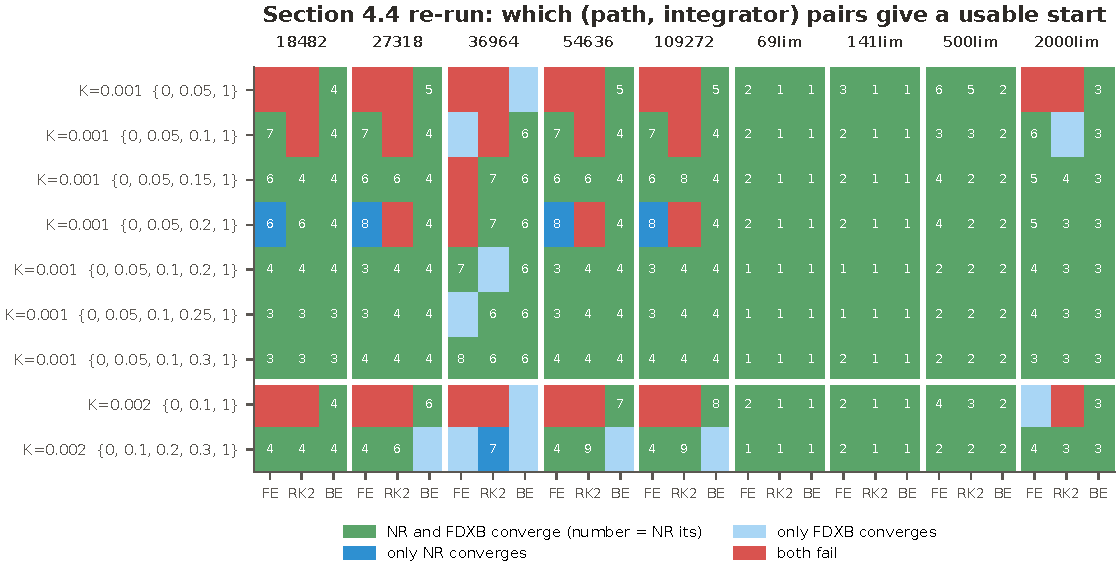
\includegraphics[width=0.95\textwidth]{figures/sec44_grid.pdf}
\caption{Section 4.4 re-run. Rows: paths and $K$; columns: system and scheme. Colour: whether NR and FDXB
converge afterwards; number: NR iterations.}
\Description{Heat-map grid of convergence outcomes.}
\label{fig:sec44}
\end{figure*}

\paragraph{Figures 4 and 5: the states themselves} Following five bus voltages of \code{case109272}
through a two-point BE path and NR (\cref{fig:fig4}), angles overshoot to about 60 degrees at $t=1$ and NR
pulls them back within one iteration; bus~6 ends at \SI{1.0045}{pu} and 21.10 degrees. The mismatch goes
$201\to25\to1.26$ along the path and $1.70\to1.7\times10^{-2}\to7.3\times10^{-7}\to8.5\times10^{-12}$ in NR:
four iterations, as the paper reports. Varying the constant step after $t_1$ (\cref{fig:fig5full}, \cref{app:extra}), smaller
steps give NR a closer start and save one NR iteration, but each extra path point costs an LU, so total cost
rises from 6 to 14 factorizations (\cref{fig:fig5}), which quantifies the paper's own conclusion.

\begin{figure}[t]
\centering
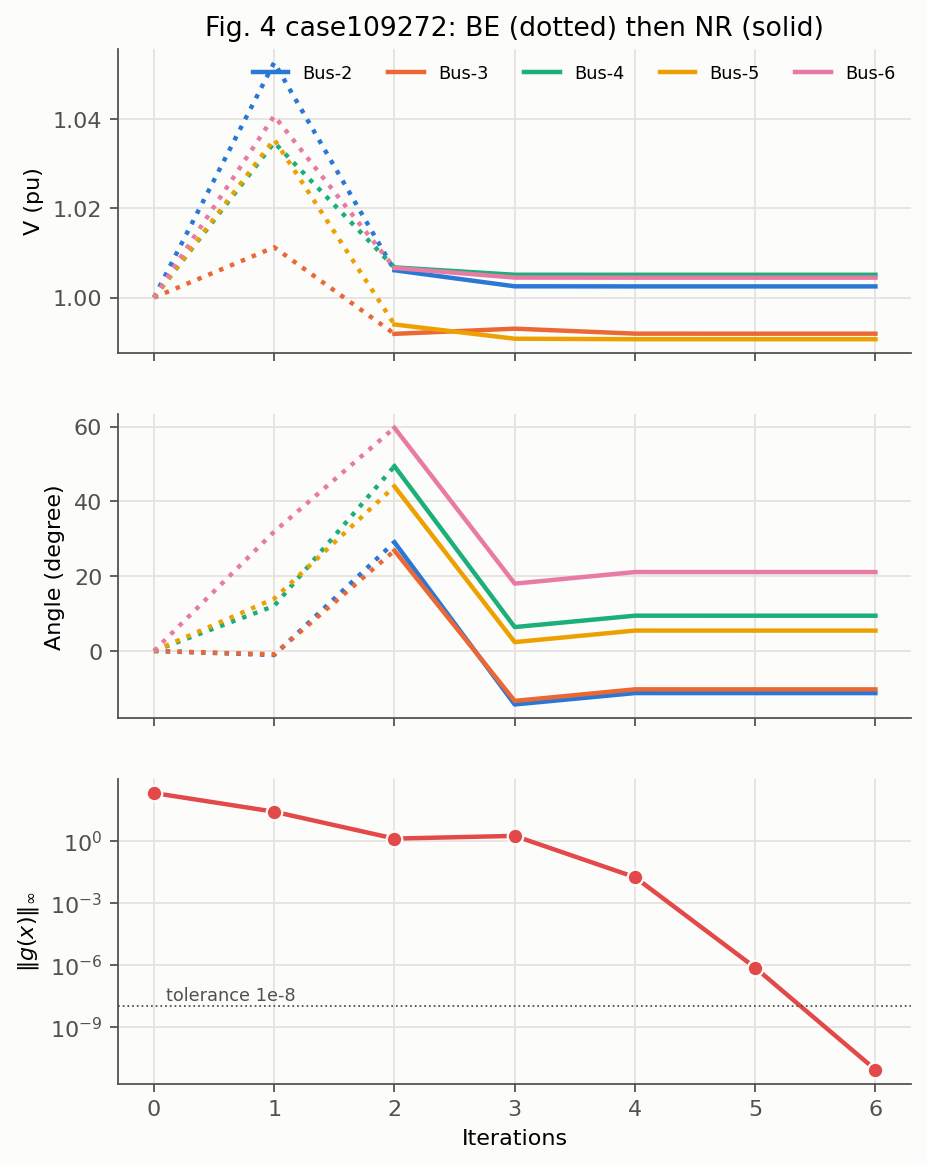
\includegraphics[width=0.95\columnwidth]{figures/repo/fig4_case109272_states.png}
\caption{Figure 4 re-run: voltage magnitudes and angles of buses 2--6 of \code{case109272} along the
two-point BE path (dotted) and NR (solid). The large angle excursion at $t=1$ is harmless: the state is
already inside NR's region of convergence.}
\Description{Line plots of bus voltages and angles over path points and NR iterations.}
\label{fig:fig4}
\end{figure}

\begin{figure}[t]
\centering
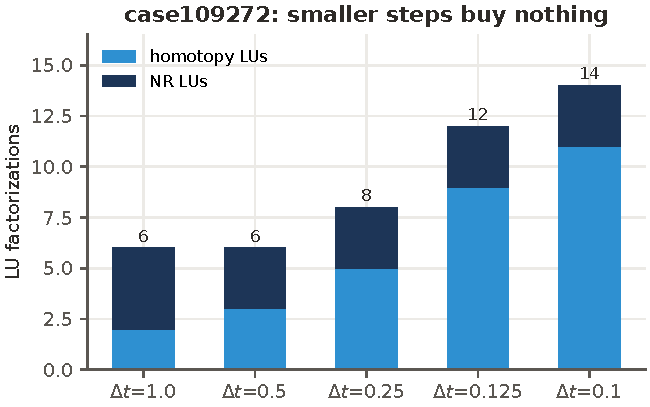
\includegraphics[width=\columnwidth]{figures/fig5_tradeoff.pdf}
\caption{Figure 5 re-run in cost terms: LU factorizations for each constant step $\Delta t$ after $t_1$.
Every run ends at the same state.}
\Description{Bar chart of LU factorizations against time step.}
\label{fig:fig5}
\end{figure}

\paragraph{Table 7: iterations} \Cref{tab:t7} is the paper's headline comparison. NR from the flat start
fails on all five ill-conditioned grids; BE(NR) needs 4 iterations and RK2(NR) 3 on all of them, and FDXB
counts match to the iteration. 54 of the 63 cells agree exactly. Six of the nine differences are the two
small limit cases, whose counts match the paper only on the stored 10\,MVA base; the others are our GSH-NR
reconstruction on two systems and one FDXB count for \code{case109272} (\cref{sec:audit}). Every converged
run in the table reaches the reference operating point.

\begin{table*}[t]
\centering
\caption{Table 7 re-run: iterations of the refining solver (ours / paper). NR-MAT starts from the case file,
all others from the flat start. BE uses the path $\{0,0.005,1\}$, RK2 the paper's path $\{0,0.005,0.01,0.02,0.12,0.42,0.72,1\}$.
Mismatches with the paper are in \textbf{bold}.}
\label{tab:t7}
\small
\setlength{\tabcolsep}{6pt}
\begin{tabular}{@{}l c c c c c c c@{}}
\toprule
\thead{Case} & \thead{NR-MAT} & \thead{NR-flat} & \thead{GSH-NR} & \thead{BE(NR)} & \thead{RK2(NR)} & \thead{BE(FDXB)} & \thead{RK2(FDXB)} \\
\midrule
\code{case18482}  & 6 / 6 & \fail\ / \fail & 10 / 10 & 4 / 4 & 3 / 3 & 33 / 33 & 29 / 29 \\
\code{case27318}  & 5 / 5 & \fail\ / \fail & \textbf{\fail\ / 25} & 4 / 4 & 3 / 3 & 29 / 29 & 25 / 25 \\
\code{case36964}  & 6 / 6 & \fail\ / \fail & \textbf{28 / 27} & 4 / 4 & 3 / 3 & 33 / 33 & 29 / 29 \\
\code{case54636}  & 5 / 5 & \fail\ / \fail & \fail\ / \fail & 4 / 4 & 3 / 3 & 29 / 29 & 25 / 25 \\
\code{case109272} & 5 / 5 & \fail\ / \fail & \fail\ / \fail & 4 / 4 & 3 / 3 & \textbf{29 / 19} & 25 / 25 \\
\code{case69limit}   & \textbf{2 / 4} & \textbf{2 / 4} & \textbf{2 / 4} & 1 / 1 & 1 / 1 & 8 / 8 & 8 / 8 \\
\code{case141limit}  & \textbf{2 / 3} & \textbf{2 / 3} & \textbf{2 / 3} & 1 / 1 & 1 / 1 & 8 / 8 & 6 / 6 \\
\code{case500limit}  & 3 / 3 & 4 / 4 & 4 / 4 & 2 / 2 & 2 / 2 & 13 / 13 & 11 / 11 \\
\code{case2000limit} & 3 / 3 & 5 / 5 & 5 / 5 & 3 / 3 & 3 / 3 & 22 / 22 & 20 / 20 \\
\bottomrule
\end{tabular}
\end{table*}

\paragraph{Table 8: run time} The timing results of Tables 6 and 8 are the medians of seven runs saved in the repository; rerunning both experiments with the current code gives identical iteration counts and failures. Relative to NR-MAT (\cref{fig:timing}), BE(FDXB) is
faster than NR-MAT on all five ill-conditioned systems, at 66--93\% of its time against the paper's
57--85\%, and BE(NR) costs slightly more (102--122\% against 92--128\%). Both conclusions of the paper hold.
RK2 is much slower for us (252--331\%) than for the paper (84--218\%): its path has seven steps after $t=0$ and every step needs two LUs, one per slope; we take that, rather than a property of Python, as the likely reason, but did not profile it. Because Python and MATLAB timings are not
comparable, our own cost comparisons use LU counts.

\begin{figure*}[t]
\centering
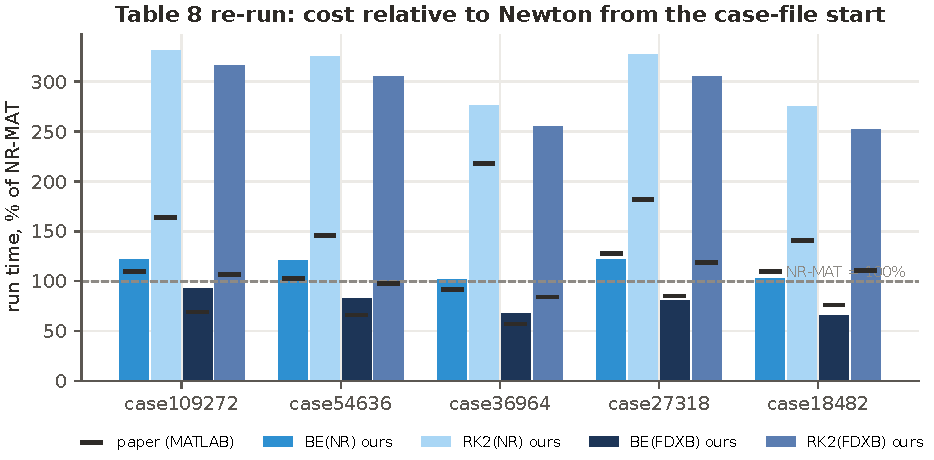
\includegraphics[width=0.85\textwidth]{figures/timing.pdf}
\caption{Table 8 re-run: median run time of seven repetitions as a percentage of NR-MAT (bars) against the
paper's MATLAB percentages (black ticks).}
\Description{Grouped bar chart of relative run times.}
\label{fig:timing}
\end{figure*}

\begin{finding}{Reproduction (Q1, Q2).}
The method works as the paper says. On all five ill-conditioned grids, a two-point BE path turns a
divergent flat start into a four-iteration NR solve, and our numbers track the paper's across 28 orders of
magnitude. Where explicit schemes fail, they fail where the paper says, for the reason
\cref{sec:firststep} gives.
\end{finding}

\subsection{Auditing the base paper}\label{sec:audit}
For every disagreement we first checked our own code; the eight in \cref{tab:audit} survived that check.
Two further conventions had to be discovered before anything matched: FDXB iterations are counted as $P$
plus $Q$ updates, and the flat start includes the slack angle. With those fixed, the base-MVA issue is the
only one that changes a conclusion, and only for the two smallest systems.

\begin{table*}[t]
\centering
\caption{Eight places where the base paper is inconsistent or under-specified, the evidence, and our handling.}
\label{tab:audit}
\footnotesize
\begin{tabularx}{\textwidth}{@{}>{\raggedright\arraybackslash}p{3.6cm} >{\raggedright\arraybackslash}X >{\raggedright\arraybackslash}p{3.6cm}@{}}
\toprule
\thead{Issue} & \thead{Evidence} & \thead{Our handling} \\
\midrule
Base MVA of \code{case69limit}, \code{case141limit} &
Files store 10\,MVA. Tables 2--5 match only on 100\,MVA; Table 7's NR-MAT/NR-flat counts (4, 3) match only on 10\,MVA, where BE(NR) then needs 2, not 1. No single base reproduces both. &
Use 100\,MVA; report 10\,MVA counts separately. \\
BE(FDXB) $=19$ for \code{case109272} (Table 7) &
We get 29, the same as \code{case54636}. The two systems are 8 and 4 copies of one network and are identical in every other cell of every table, the paper's included. &
Reported; most likely a typo. \\
Table 2, FE on \code{case18482} at $t=0.01$ &
Paper 9.7, ours 3.7; every other cell of that column matches to two digits. &
Reported, unresolved. \\
Fig.~1(a), $\epsilon=0.05$ &
One NR step from $(1,0.95)$ gives $x=(6.01,-4.01)$ and $\ninf{g}\approx 99.5$, i.e.\ $\log_{10}\approx2$; the paper's curve starts near 3. We need 8 iterations, not 9. &
Computed by hand and in code. \\
GSH-NR specification &
Described in words only; no formula for the shunts or for $\delta$. Our reconstruction matches \code{case18482} (10) and nearly \code{case36964} (28 vs 27) but fails on \code{case27318} (paper: 25). &
Our version documented in \code{gsh.py}. \\
Section 4.4, $\Delta t_0=0.1$ &
``Does not work'' is stated without the path used. With $\{0,0.1,1\}$ BE works on 8 of 9 systems; with $\{0,0.1,0.2,0.3,1\}$ it fails on the four largest with NR. &
Both paths reported (\cref{fig:sec44}). \\
Table 6, RK2, $t_3=0.20$, \code{case36964} &
The paper reports success (232\%); in our run RK2 diverges on this path. &
Reported. \\
Flat-start mismatch of \code{case2000limit} &
Tables 2--4 print 54, Table 5 prints 55 for the same starting point (ours: 54.95). &
Cosmetic; rounding. \\
\bottomrule
\end{tabularx}
\end{table*}

\subsection{Results of the modifications}\label{sec:modresults}

\paragraph{First, which root?}\label{sec:rootcheck}
On the 170 runs of the test bed, the paper's method gives NR a start from which it converges 141 times. But
14 of those runs converge to a \emph{different} solution than the reference: \code{case54636} and
\code{case109272} in S3, S4 and S5, \code{case27318} in S4 and S5, \code{case3012wplimit} in S1 and S2,
\code{case3375wplimit} in S1, S2 and S3, and \code{case13659pegaselimit} in S4. The mismatch is below
$10^{-8}$ in all of them; only comparing the voltages tells them apart. In the paper's own setting S1 all
nine of the paper's systems reach the reference, and so does every converged run of our Table~7 re-run,
which checks it; but on the wider test bed the method truly solves 127 of 170 runs, not 141.

\paragraph{Headline numbers} \Cref{tab:improve} and \cref{fig:solved} give all 2{,}890 runs. Every
configuration that contains the corrector solves 152 and loses nothing; the multiplier alone solves 143;
Richardson control solves 145--158 depending on the step rule. The four other ideas lose runs, fixed-step
RK4 catastrophically. \Cref{fig:pareto} plots robustness against cost: multiplier plus corrector is both
more robust \emph{and} cheaper than the paper's method; the corrector alone is as robust at about 5\% more
LUs; Richardson control costs 18--30\% more with BE and 4--8 times more with FE, RK2 and RK4.

\begin{table*}[t]
\centering
\caption{Runs that reach the reference solution (of 34 per setting, 170 in total). \emph{Other}: runs that
converge to a different root. \emph{Gained}/\emph{lost} are relative to the paper's method, with gains split
into rescues / root fixes / speed-ups. \emph{LUs S1}: mean factorizations in S1 on the systems both this
configuration and the paper's method solve (the paper's own mean on those systems in grey where it is not
8.04). \emph{Ratio}: the same, all settings pooled, relative to the paper's method.}
\label{tab:improve}
\footnotesize
\setlength{\tabcolsep}{4.5pt}
\begin{tabular}{@{}l r r r r r r r l r l r@{}}
\toprule
\thead{Configuration} & \thead{S1} & \thead{S2} & \thead{S3} & \thead{S4} & \thead{S5} & \thead{Total} & \thead{Other} & \thead{Gained} & \thead{Lost} & \thead{LUs S1} & \thead{Ratio} \\
\midrule
\rows{generated/improve_table.tex}
\bottomrule
\end{tabular}
\end{table*}

\begin{figure*}[t]
\centering
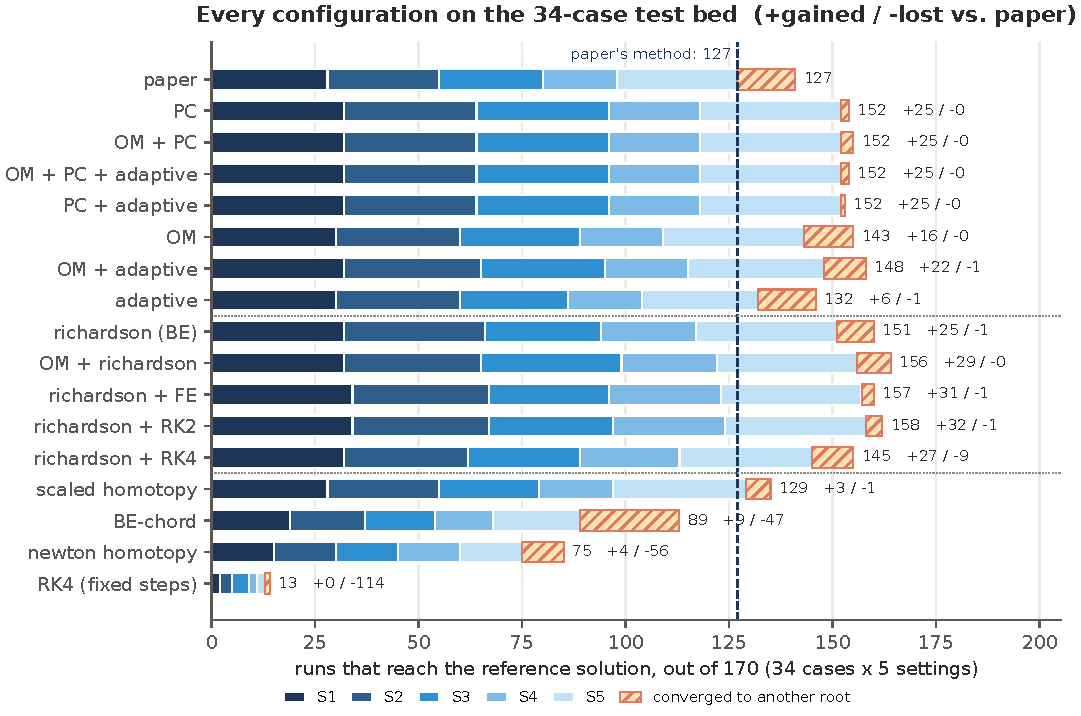
\includegraphics[width=0.92\textwidth]{figures/improve_solved.pdf}
\caption{Runs that reach the reference solution per configuration, stacked by setting; hatched: runs that
converge to another root. Dashed line: the paper's method.}
\Description{Stacked bar chart of solved runs per configuration.}
\label{fig:solved}
\end{figure*}

\begin{figure*}[t]
\centering
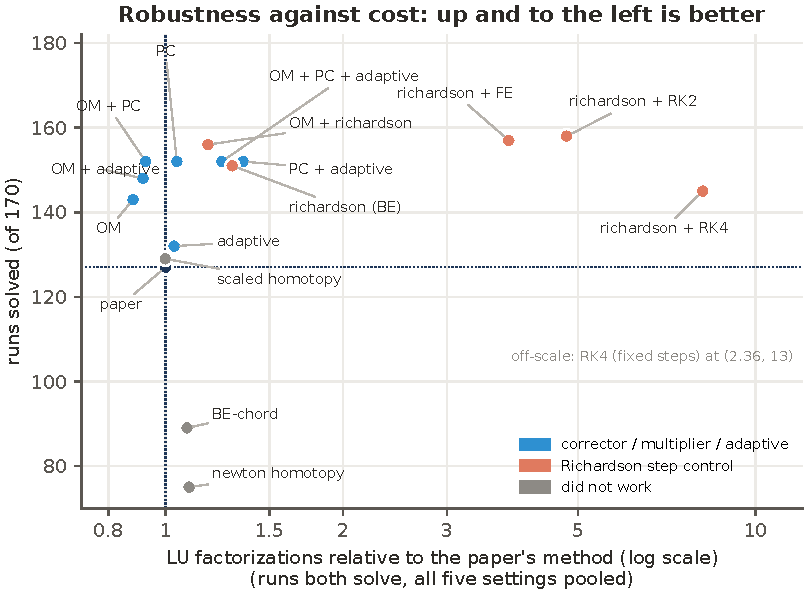
\includegraphics[width=0.55\textwidth]{figures/improve_pareto.pdf}
\caption{Runs solved against LU cost relative to the paper's method (log scale). Blue: corrector,
multiplier, adaptive and combinations; orange: Richardson control; grey: the four ideas that did not work.}
\Description{Scatter plot of robustness against cost.}
\label{fig:pareto}
\end{figure*}

\begin{finding}{The corrector is the robust improvement, the multiplier the cheap one (Q4).}
The Newton corrector alone solves 25 more runs than the paper's method (2 rescues, 13 wrong roots corrected,
10 speed-ups), never loses one, and cuts the other-root runs from 14 to 2, for 0.4 more LUs per system in S1
(8.43 against 8.04). The optimal multiplier alone is 11\% cheaper (7.14 LUs) but still lands on another root
12 times. Together, multiplier plus corrector keeps all of the corrector's robustness (152 solved, no losses)
and most of the multiplier's saving (7.57 LUs in S1, 7\% fewer than the paper's method over all settings).
It is the configuration we recommend.
\end{finding}

\paragraph{Richardson step control} Error-controlled steps are the only change that solves some runs nothing
else solves: \code{case6024} in S1 (73 LUs with BE), and \code{case7092}, \code{case10595} and \code{case12110}
with the weak $K$ of S4. Multiplier plus Richardson rescues 10 of the 11 divergent runs of the test bed, more
than any other configuration, and solves 156 runs without losing one. On \code{case6024}
(\cref{fig:richardson}) the paper's jump from $t_1$ to $t=1$ lands where NR cannot recover; the controller
forces small steps early, where the state changes fastest, and lets them grow later. The study also tests the
paper's preference for BE under fair, error-controlled conditions, and it holds: in S1 Richardson control needs
10.6 LUs with BE, 37 with FE, 48 with RK2 and 87 with RK4.

\begin{figure*}[t]
\centering
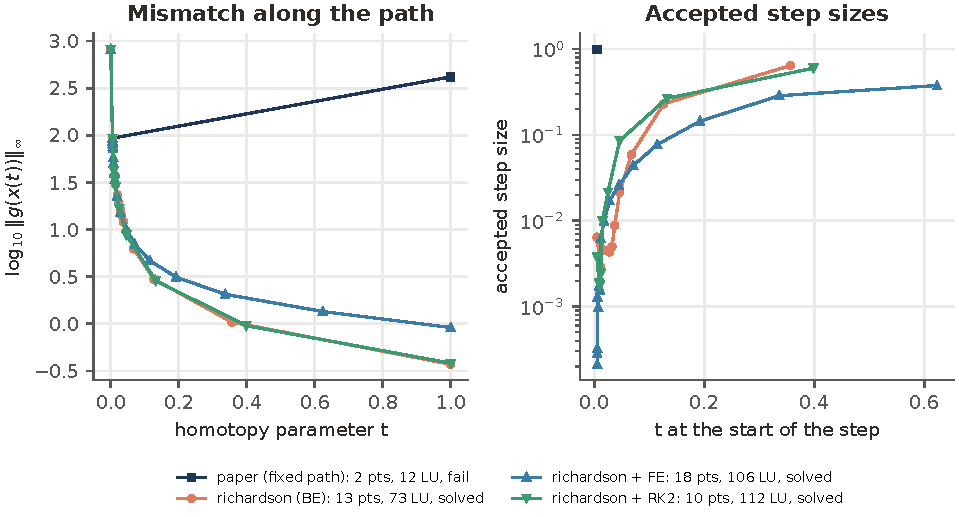
\includegraphics[width=0.9\textwidth]{figures/richardson_path.pdf}
\caption{Richardson-controlled paths on \code{case6024}, setting S1, the one S1 system only Richardson
control solves. Left: mismatch at each accepted point (legend: points, LUs including rejected attempts, and
outcome). Right: accepted step sizes.}
\Description{Two plots of mismatch and step size along Richardson-controlled paths.}
\label{fig:richardson}
\end{figure*}

\paragraph{System by system, and the nature of the gains} On the paper's nine systems little changes in S1
(\cref{fig:cases}, \cref{app:extra}): the method already works with 3--6 LUs. The differences are on the added systems: the
multiplier saves one to three LUs on 13 of the 14 extra limit cases that both it and the paper's method
solve, and on \code{case3012wplimit} and \code{case3375wplimit} every configuration with the corrector reaches
the reference (9--11 LUs) where the paper's method finds another root. Of the 36 runs the paper's method does
not solve but some configuration does, 10 are \emph{speed-ups} (\code{case14limit} and \code{case2736splimit}
in all five settings: the paper's method needs 11 NR iterations, one over budget), 15 are \emph{root fixes}
(13 of them by the corrector; the other two, \code{case109272} and \code{case13659pegaselimit} in S4, by
Richardson control with an explicit step rule, and the latter also by BE-chord) and 11 are true
\emph{rescues} (the paper's method diverges even with 30 NR iterations), of which multiplier plus Richardson
rescues 10, Richardson with BE 9, multiplier plus adaptive 4, the corrector 2 and the multiplier 1
(\cref{fig:rescues}). The adaptive rule solves \code{case6748}, which the paper's fixed path
cannot, by halving the jump six times and then doubling its way to $t=1$ (\cref{fig:adaptive}); both runs are drawn in \cref{app:extra}.

\subsection{Results of the numerical studies}\label{sec:proposal}

\paragraph{Spectrum} On the twelve ill-conditioned systems $|\lambda|_{\min}(J(\xo))$ is $4\times10^{-4}$ to
$6\times10^{-3}$ while $|\lambda|_{\max}$ is $2.7$--$5.2\times10^{4}$, so the eigenvalue ratio reaches
$1.2\times10^{8}$ (\code{case109272}). The paper's $\delta=0.02$ lifts the smallest eigenvalue to 0.020--0.026
and cuts the ratio by a factor of 4 to 52, to $1.1$--$2.3\times10^{6}$ on all twelve (\cref{fig:spectrum}).
On 20 of the 22 limit cases the smallest eigenvalue is already 0.012 to 1.9, comparable to the shift or larger,
so the shift changes their spectrum little. The two exceptions are the limit cases built from the two largest
PEGASE grids, \code{case9241pegaselimit} ($4.9\times10^{-3}$) and \code{case13659pegaselimit}
($4.8\times10^{-4}$), whose spectrum looks like that of the ill-conditioned systems. Inverse iteration agrees
with ARPACK to four digits on 33 of the 34 systems; on \code{case57limit} it returns 0.2467 against ARPACK's
0.2273. The power method is less reliable: its error exceeds 5\% on four systems, \code{case18482} (13\%),
\code{case36964} (8\%), \code{case10595} (19\%) and \code{case12110} (13\%), all of which contain the
9241-bus PEGASE network, and it is 1.9\% and 2.9\% off on \code{case\_ieee30limit} and
\code{case9241pegaselimit}. The power method converges slowly when the two largest eigenvalue moduli are
close; we did not measure that gap, so this is the likely, not a proven, cause.

\begin{figure*}[t]
\centering
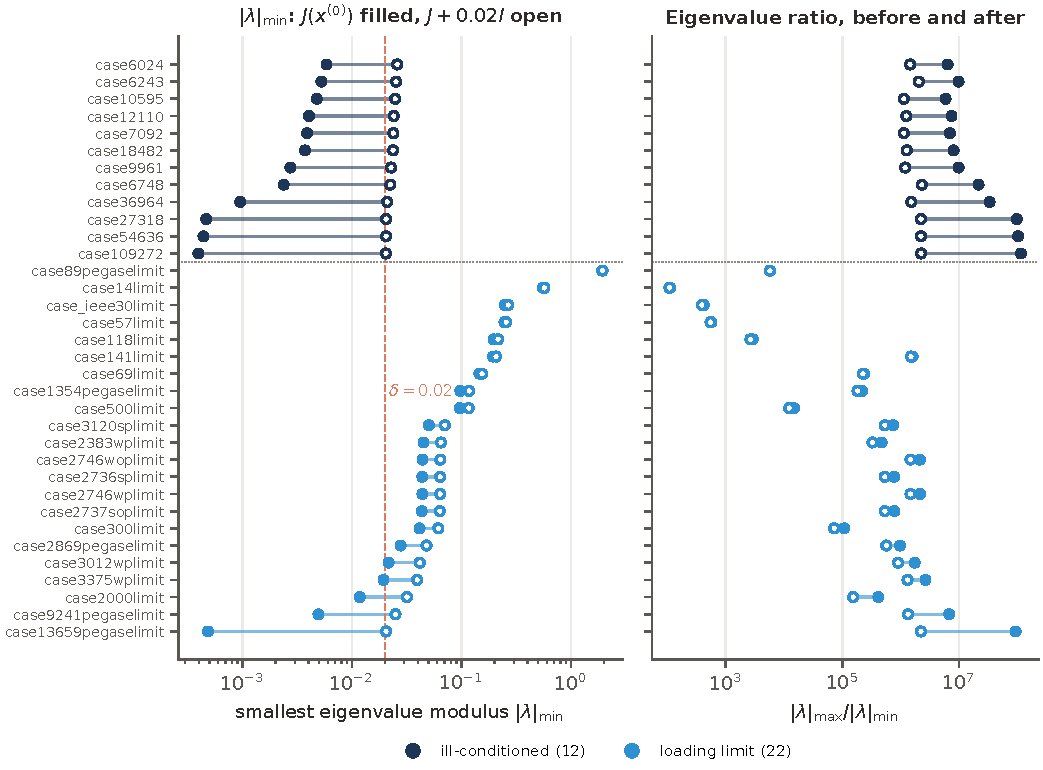
\includegraphics[width=0.92\textwidth]{figures/spectrum.pdf}
\caption{Smallest eigenvalue modulus (left) and $|\lambda|_{\max}/|\lambda|_{\min}$ (right) of $J(\xo)$
(filled) and of $J+0.02I$ (open) for all 34 systems. The shift matters only where $|\lambda|_{\min}<\delta$.}
\Description{Two dot plots of eigenvalue statistics per system.}
\label{fig:spectrum}
\end{figure*}

\paragraph{Feasibility maps} The method works in a band along the diagonals $\delta=\text{const}$
(\cref{fig:feasibility}), which confirms that $\delta$, not $K$ or $\Delta t_0$ alone, is the parameter that
matters. The band's width depends on the system: almost the whole grid works for \code{case18482} and
\code{case2000limit}, but only 29 of 88 cells for \code{case36964}, with no cell at $\Delta t_0=0.1$ or 0.2,
which explains the paper's finding that $\Delta t_0=0.1$ fails although $\delta$ is unchanged. For
\code{case6024} the band lies at $\delta$ from 0.03 to 32, and the paper's $\delta=0.02$ runs along its edge.

\begin{figure*}[t]
\centering
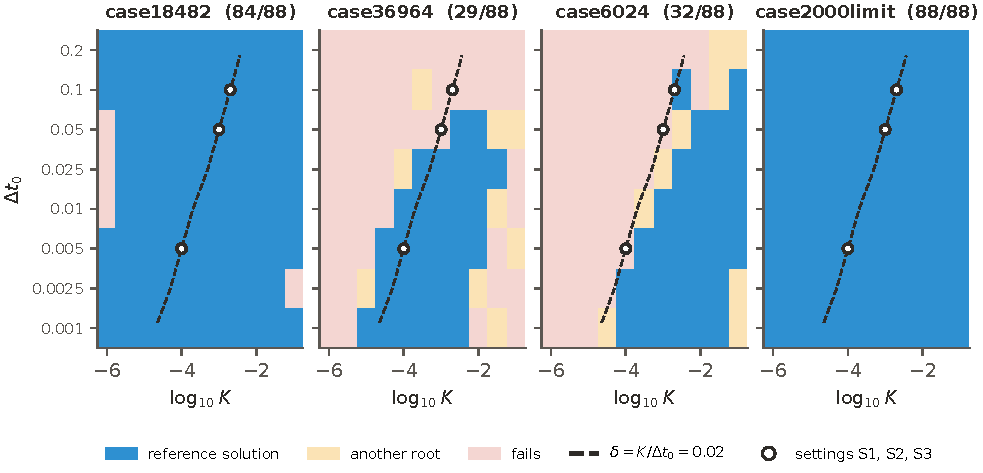
\includegraphics[width=0.92\textwidth]{figures/feasibility.pdf}
\caption{Outcome of the paper's method on a grid of $K$ and $\Delta t_0$. Dashed: $\delta=0.02$, the paper's
shift. Circles: settings S1, S2 and S3.}
\Description{Four outcome maps over the K and dt0 plane.}
\label{fig:feasibility}
\end{figure*}

\paragraph{Tuning $\delta$} For \code{case27318}, \code{case54636} and \code{case109272} golden-section
search lands at $\delta=0.025$, close to the paper's 0.02. On \code{case36964} it lands at 0.096, and on the
other eight ill-conditioned systems at 1.0 to 4.8, fifty or more times the paper's value. On 12 of the 22
limit cases it runs to the lower end of the interval ($\delta\approx10^{-4}$), because there $\delta$ hardly
changes the LU count (\cref{fig:tuning}). Rules fitted on the paper's nine systems and tested on the other 25 (\cref{tab:tuning})
show that a fixed $\delta=0.011$ behaves like the paper's 0.02, a spectral rule $\delta=c\,|\lambda|_{\min}$
fails (it loses four of nine training systems; the tuned $\delta$ is 54 to 819 times $|\lambda|_{\min}$), and a
per-system search solves four more test systems but costs 21 solves, far more than it saves.

\begin{figure*}[t]
\centering
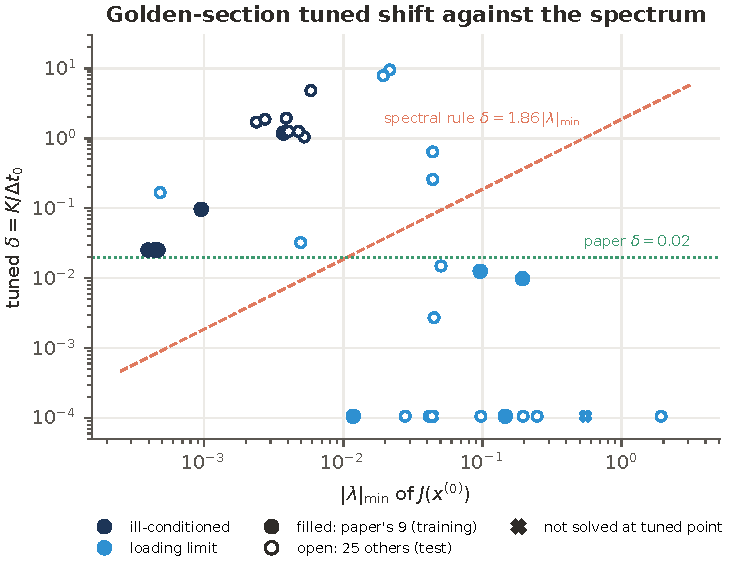
\includegraphics[width=0.5\textwidth]{figures/tuning.pdf}
\caption{Golden-section tuned $\delta$ against $|\lambda|_{\min}(J(\xo))$. Points at $10^{-4}$: the search ran
to the lower end because $\delta$ does not matter. A spectral rule would put the points on a line of slope one.}
\Description{Scatter plot of tuned delta against smallest eigenvalue modulus.}
\label{fig:tuning}
\end{figure*}

\begin{table}[t]
\centering
\caption{Choosing $\delta$ without a search: rules fitted on the paper's nine systems, tested on the other
25. Mean LUs are over solved systems and exclude the search itself.}
\label{tab:tuning}
\footnotesize
\setlength{\tabcolsep}{3pt}
\begin{tabular}{@{}>{\raggedright\arraybackslash}p{2.9cm} c r c r@{}}
\toprule
\thead{How $\delta$ is chosen} & \thead{Train} & \thead{LUs} & \thead{Test} & \thead{LUs} \\
\midrule
paper, $\delta=0.02$ & 9/9 & 5.00 & 19/25 & 9.47 \\
fixed, $\delta=0.011$ & 9/9 & 5.11 & 19/25 & 9.53 \\
spectral, $\delta=1.86\,|\lambda|_{\min}$ & \textbf{5/9} & 5.20 & 20/25 & 11.00 \\
golden search per system (21 solves) & 9/9 & 4.89 & \textbf{23/25} & 9.13 \\
\bottomrule
\end{tabular}
\end{table}

\paragraph{Own LU} On the tutorial and the limit cases of 69 to 2{,}000 buses our dense LU gives exactly the
same iteration counts as SuperLU and the same solution to $5\times10^{-12}$ (\cref{tab:ownlu}). The time shows
why the paper's systems need a sparse solver: NR on \code{case2000limit} takes \SI{424}{s} with our LU against
\SI{0.04}{s} with SuperLU, and the dense Jacobian of \code{case109272} alone would need about \SI{276}{GB}.
Reusing factors also matters: for 20 right-hand sides with one $400\times400$ matrix, one LU plus 20 pairs of
triangular solves is 14 times faster than 20 Gauss eliminations, which is why FDXB factorises $B'$ and $B''$
once.

\begin{table*}[t]
\centering
\caption{The paper's method (BE path $\{0,0.005,1\}$, $K=10^{-4}$) with SciPy's sparse LU and with our dense
LU with partial pivoting: refiner iterations, largest difference in the solution, and run time.}
\label{tab:ownlu}
\small
\setlength{\tabcolsep}{7pt}
\begin{tabular}{@{}l l r r r r r@{}}
\toprule
\thead{System} & \thead{Refiner} & \thead{Its SuperLU} & \thead{Its ours} & \thead{max $|\Delta x|$} & \thead{SuperLU (s)} & \thead{Ours (s)} \\
\midrule
tutorial  & NR   & 9  & 9  & 0             & 0.002 & 0.002 \\
\code{case69limit}   & NR   & 1  & 1  & $3.6\times10^{-13}$ & 0.004 & 0.011 \\
                     & FDXB & 8  & 8  & $1.6\times10^{-13}$ & 0.004 & 0.010 \\
\code{case141limit}  & NR   & 1  & 1  & $9.7\times10^{-14}$ & 0.005 & 0.039 \\
                     & FDXB & 8  & 8  & $4.7\times10^{-12}$ & 0.004 & 0.032 \\
\code{case500limit}  & NR   & 2  & 2  & $9.8\times10^{-15}$ & 0.010 & 3.45 \\
                     & FDXB & 13 & 13 & $1.2\times10^{-14}$ & 0.008 & 1.71 \\
\code{case2000limit} & NR   & 3  & 3  & $4.3\times10^{-14}$ & 0.040 & 424.1 \\
                     & FDXB & 22 & 22 & $6.2\times10^{-14}$ & 0.029 & 100.8 \\
\bottomrule
\end{tabular}
\end{table*}

\begin{finding}{Numerical studies (Q5).}
The shift $\delta$ matters exactly where the spectrum says it should: on systems whose flat-start Jacobian
has eigenvalues below $\delta$. There the method works in a band of constant $\delta$ whose position depends
on the system, and neither a fixed value nor a multiple of $|\lambda|_{\min}$ predicts the best $\delta$.
This is why the corrector, which makes more settings work instead of looking for a better one, is worth more
than tuning $\delta$.
\end{finding}

\subsection{Discussion: why the failures fail}\label{sec:failure}
\paragraph{Explicit schemes} FE at $t=0$ steps by $-(\Delta t_0/K)\,g(\xo)$, blind to the network, and
later explicit steps to $t=1$ still use $G_x$ at $t_1$, dominated by $KI$ wherever $J$ is small. The ODE is
stiff in the sense of~\cite{hairer1996}: its fast modes have time scale $K/|\lambda(J)|$, which with
$|\lambda|$ from $4\times10^{-4}$ to $5\times10^{4}$ (\cref{fig:spectrum}) spans eight orders of magnitude.
An explicit method is stable only for steps of the order of the fastest of these time scales, while an
implicit one is not restricted in this way~\cite{hairer1996}. RK4 is explicit, which is consistent with its
failure with fixed steps (13 of 170 runs). Under Richardson control it solves 145 runs but needs 87 LUs per
system in S1 against 37 for FE and 10.6 for BE: every attempt costs twelve LUs (three steps of four stages),
and its higher order does not buy larger steps. Our reading is that the steps are limited by stability rather
than accuracy; we did not measure the accepted RK4 step sizes.

\paragraph{BE-chord} Its fixed-point iteration has derivative
\[
  -\Delta t\,G_x(x_k,t_{k+1})^{-1}\bigl(J(\hat x)-KI\bigr).
\]
On the last step $G_x=J(x_k)$, so when $J(\hat x)\approx J(x_k)$ the iteration matrix is close to
$-\Delta t\,I$ with $\Delta t=0.995$: its spectral radius is about one, so the iteration does not contract.
The first iterate is the BE step itself; the second and third can only move away from it. BE-chord loses 47
runs and lands on another root 24 times. This is our analysis of why it fails; we measured the outcome, not
the spectral radius.

\paragraph{Newton and scaled homotopies} The Newton homotopy has $G_x=J(x)$ at every $t$ and no $KI$ term;
its BE first step is $-\Delta t_0\,J(\xo)^{-1}g(\xo)$, a plain Newton step shrunk to $\Delta t_0$ (0.5\% in
S1) with the flat-start Jacobian unregularised. It solves only 75 of 170 runs; in S1 it fails on every
ill-conditioned system except \code{case27318} and \code{case54636}, and on \code{case109272} it reaches
another root. This is the clearest evidence in the project that the useful ingredient is the $KI$ shift, not
continuation as such. The scaled homotopy solves 129 runs against the paper's 127: the same as the paper in
S1, S2 and S4, one fewer in S3 (\code{case27318}) and three more in S5, all three root fixes. Since $D$ is
normalised to mean one, equations with a small Jacobian diagonal get a \emph{smaller} shift than in the
paper's method; our interpretation is that this is why it does not help more.

\paragraph{Accounting and acceptance tests} At $t=1$ the corrector's step is exactly one NR step taken
before the 10-iteration budget starts counting, so 10 of its 25 gains are budget-edge speed-ups; the other 15
(two rescues and 13 root fixes) are real. The adaptive rule accepts a step only if $\ninf{g}$ decreases, but on
the path $g(x(t))=-\tfrac{1-t}{t}K(x(t)-\xo)$ need not fall monotonically, so it rejects good steps (14 LUs
instead of 5 on \code{case2000limit}). Richardson control compares two integrations with each other, not with
the homotopy curve, so both can drift towards another branch (9 wrong roots with BE, against 2 for the
corrector).

\paragraph{Strengths of this study} Every number in this report is produced by a script in the repository,
and every reproduced value is printed next to the paper's; the building blocks are tested before any
comparison; the algebra of \cref{sec:firststep} is consistent with which modifications work (those that
improve the Newton stages) and which fail (the one that removes the shift); and the modification study is a
controlled experiment on 34 systems with a machine-independent cost and a root check. Seven runs, all with the
weak $K$ of S4 (\code{case36964}, \code{case6024}, \code{case6243}, \code{case6748}, \code{case9961},
\code{case3012wplimit}, \code{case3375wplimit}), are solved by no configuration.

%% ============================================================================ 5 CONCLUSION
\clearpage
\section{Conclusion and Future Work}\label{sec:conclusion}
\paragraph{Key takeaways} The base paper reproduces: on all five ill-conditioned grids of up to 109{,}272
buses NR from the flat start fails, and a two-point backward-Euler homotopy turns that into a
four-iteration solve, with our numbers matching the paper's across 28 orders of magnitude. The method is
simpler than its derivation suggests: the first BE step is a Newton step on a Jacobian shifted by
$\delta=K/\Delta t_0$ and the second is almost a plain Newton step; BE wins because it is the only scheme
that uses the real Jacobian where it matters. On a test bed four times the paper's, the most important
question turned out to be \emph{which solution} a converged run reaches: the paper's method converges on 141
of 170 runs but reaches the intended operating point on 127. A Newton corrector raises that to 152 and cuts
wrong-root runs from 14 to 2; with Iwamoto's optimal multiplier it does so with 7\% fewer LU factorizations,
and this is the configuration we recommend. Richardson control solves systems nothing else solves at 18--30\%
more cost and confirms under fair conditions that BE is the right integrator. The shift matters where the
flat-start Jacobian has eigenvalues below it, and no fixed or spectral rule predicts its best value.

\paragraph{Limitations} The test bed is two Zenodo records, and the ill-conditioned systems are replicas of a
few base networks, so they carry less independent evidence than unrelated grids would. The reference
operating point is a convention (the root NR reaches from the stored guess), and we did not study whether the
other roots are physically meaningful. The modification study used only paths $\{0,\Delta t_0,1\}$; the
Richardson tolerance and golden-section brackets were set once and not tuned; the feasibility maps cover four
systems; our GSH-NR is a reconstruction from a verbal description; and timings are noisy Python measurements on
a laptop.

\paragraph{Future work} (i)~A Richardson path with a corrector after each accepted point, to combine the
most rescues with the fewest wrong roots. (ii)~Cheaper error estimates, through an embedded pair or one LU
reused for the three steps of each attempt, which would cut Richardson's cost by up to three times. (iii)~A
path-aware acceptance test for adaptive steps based on $\norm{G(x,t)}$ instead of $\norm{g(x)}$. (iv)~A scaling
that raises the shift on weakly coupled equations. (v)~A sparse LU from scratch with a fill-reducing ordering,
to run the whole pipeline on our own linear algebra.

\begin{acks}
We thank our course teacher, Anup Halder Joy (Department of CSE, BUET), for guidance throughout the CSE~402
Numerical Analysis Sessional, and the authors of the base paper and of the Zenodo test-system records for
making their work public.
\end{acks}

%% ============================================================================ REFERENCES
\bibliographystyle{ACM-Reference-Format}
\bibliography{references}

%% ============================================================================ APPENDIX
\clearpage
\onecolumn
\appendix
\section{Reproducing This Report}\label{app:repro}
All results come from the public repository~\cite{ourrepo} (\repo). Test systems are downloaded from Zenodo
on first use. Experiments 1--10 (the paper) take about an hour on a laptop; experiment 11 (17 configurations
$\times$ 170 runs) takes several hours.
\begin{lstlisting}[style=sh]
pip install -r requirements.txt
python -m pytest tests                  # 24 tests
python run_all.py                       # every experiment (1-15)
python run_all.py --only 3 4            # selected experiments
python -m improvements case36964 --corrector --multiplier
python -m improvements case6024 --richardson --dt0 0.05 --K 1e-3
python -m improvements spectrum case18482
python -m improvements feasibility case6024
python -m improvements tune case6024
python -m improvements scratch case_ACTIVSg500limit --refiner FDXB
python report/scripts/figures_from_results.py
python report/scripts/figures_from_code.py
\end{lstlisting}

\begin{table*}[!htbp]
\centering
\caption{Map from each result to the script that produces it and its output in \code{results/}.}
\label{tab:scripts}
\small
\begin{tabular}{@{}l l l@{}}
\toprule
\thead{Result} & \thead{Script} & \thead{Output} \\
\midrule
Figures 1 and 2 & \code{exp01\_tutorial.py} & \code{fig1*.png}, \code{fig2*.png} \\
Section 4.2.1 & \code{exp02\_first\_step.py} & \code{sec421\_first\_step.md} \\
Tables 2, 3, 4 & \code{exp03\_tables2to4.py} & \code{table2\_FE.md}, \code{table3\_RK2.md}, \code{table4\_BE.md} \\
Table 5 & \code{exp04\_table5.py} & \code{table5.md} \\
Section 4.4 & \code{exp05\_sec44\_pathways.py} & \code{sec44\_pathways.md} \\
Figure 3, Table 6 & \code{exp06\_fig3\_table6.py} & \code{fig3*.png}, \code{table6.md} \\
Figure 4 & \code{exp07\_fig4.py} & \code{fig4\_case109272\_states.png} \\
Figure 5 & \code{exp08\_fig5.py} & \code{fig5\_timestep\_sensitivity.png} \\
Table 7 & \code{exp09\_table7.py} & \code{table7.md}, \code{table7\_native\_base.md} \\
Table 8 & \code{exp10\_table8.py} & \code{table8.md} \\
Modifications & \code{exp11\_improvements.py} & \code{improvements\_*.md} \\
Spectrum & \code{exp12\_spectrum.py} & \code{spectrum.md} \\
$(K,\Delta t_0)$ maps & \code{exp13\_feasibility.py} & \code{feasibility.md} \\
Tuning $\delta$ & \code{exp14\_tuning.py} & \code{tuning\_per\_case.md}, \code{tuning\_rules.md} \\
Own LU & \code{exp15\_scratch\_lu.py} & \code{scratch\_lu.md}, \code{gauss\_vs\_lu.md} \\
\bottomrule
\end{tabular}
\end{table*}

\FloatBarrier
\section{Full Tables}\label{app:tables}

\begin{table*}[!htbp]
\centering
\caption{Table 2 re-run: FE after a BE first step, path $\{0,0.005,0.01,0.51,1\}$, $K=10^{-4}$ (our value
above the paper's).}
\label{tab:fe}
\scriptsize
\setlength{\tabcolsep}{4pt}
\begin{tabular}{@{}l l r r r r r r r r l@{}}
\toprule
\thead{Case} & & \thead{$t{=}0$} & \thead{0.005} & \thead{0.01} & \thead{0.51} & \thead{1} & \thead{NR 1} & \thead{NR 2} & \thead{NR 3} & \thead{Result} \\
\midrule
\rows{generated/table2_rows.tex}
\bottomrule
\end{tabular}
\end{table*}

\begin{table*}[!htbp]
\centering
\caption{Table 3 re-run: RK2 after a BE first step, same path and $K$.}
\label{tab:rk2}
\scriptsize
\setlength{\tabcolsep}{4pt}
\begin{tabular}{@{}l l r r r r r r r r l@{}}
\toprule
\thead{Case} & & \thead{$t{=}0$} & \thead{0.005} & \thead{0.01} & \thead{0.51} & \thead{1} & \thead{NR 1} & \thead{NR 2} & \thead{NR 3} & \thead{Result} \\
\midrule
\rows{generated/table3_rows.tex}
\bottomrule
\end{tabular}
\end{table*}

\begin{table*}[!htbp]
\centering
\caption{Table 6 re-run: median CPU time of seven runs as a percentage of NR-MAT, with NR iterations after
the homotopy in brackets (ours / paper).}
\label{tab:t6}
\footnotesize
\setlength{\tabcolsep}{6pt}
\begin{tabular}{@{}l c l l l@{}}
\toprule
\thead{Method} & \thead{$t_3$} & \thead{\code{case109272}} & \thead{\code{case36964}} & \thead{\code{case2000limit}} \\
\midrule
NR-MAT & -- & 1.784\,s (100\%) & 0.797\,s (100\%) & 0.024\,s (100\%) \\
\midrule
FE  & 0.20 & 143\% [3] / 146\% & 185\% [7] / 178\% & 272\% [4] / 68\% \\
FE  & 0.25 & 143\% [3] / 145\% & \fail\ / \fail & 272\% [4] / 75\% \\
FE  & 0.30 & 164\% [4] / 170\% & 201\% [8] / 179\% & 239\% [3] / 72\% \\
RK2 & 0.20 & 225\% [4] / 230\% & \textbf{\fail\ / 232\%} & 341\% [3] / 82\% \\
RK2 & 0.25 & 224\% [4] / 226\% & 222\% [6] / 190\% & 340\% [3] / 84\% \\
RK2 & 0.30 & 224\% [4] / 237\% & 221\% [6] / 195\% & 342\% [3] / 73\% \\
BE  & 0.20 & 163\% [4] / 171\% & 168\% [6] / 144\% & 238\% [3] / 61\% \\
BE  & 0.25 & 164\% [4] / 171\% & 169\% [6] / 144\% & 237\% [3] / 81\% \\
BE  & 0.30 & 163\% [4] / 169\% & 170\% [6] / 148\% & 238\% [3] / 94\% \\
\bottomrule
\end{tabular}
\end{table*}

\FloatBarrier
\section{Additional Figures and Tables}\label{app:extra}
This appendix collects the remaining reproduced figures and tables of the base paper and the
detailed per-system results of the modification study referred to in \cref{sec:results}.

\begin{figure*}[!htbp]
\centering
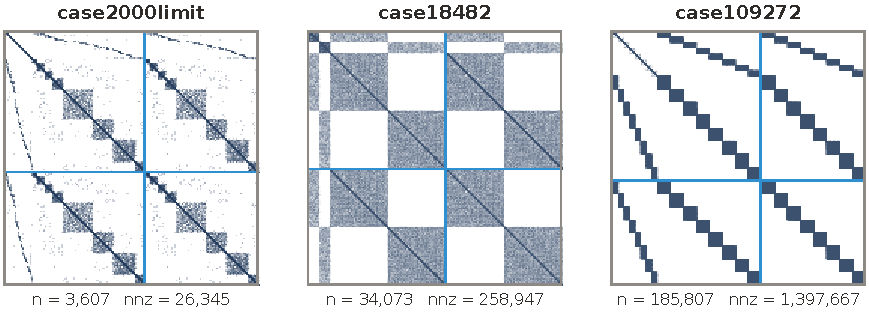
\includegraphics[width=0.92\textwidth]{figures/spy.pdf}
\caption{Nonzero pattern of the flat-start Jacobian. Orange lines separate angle from magnitude unknowns,
showing the four blocks $\partial P/\partial\theta$, $\partial P/\partial V$, $\partial Q/\partial\theta$,
$\partial Q/\partial V$. The ill-conditioned systems are copies of one network on the diagonal.}
\Description{Sparsity plots of three Jacobians.}
\label{fig:spy}
\end{figure*}

\begin{figure*}[!htbp]
\centering
\begin{subfigure}{0.325\textwidth}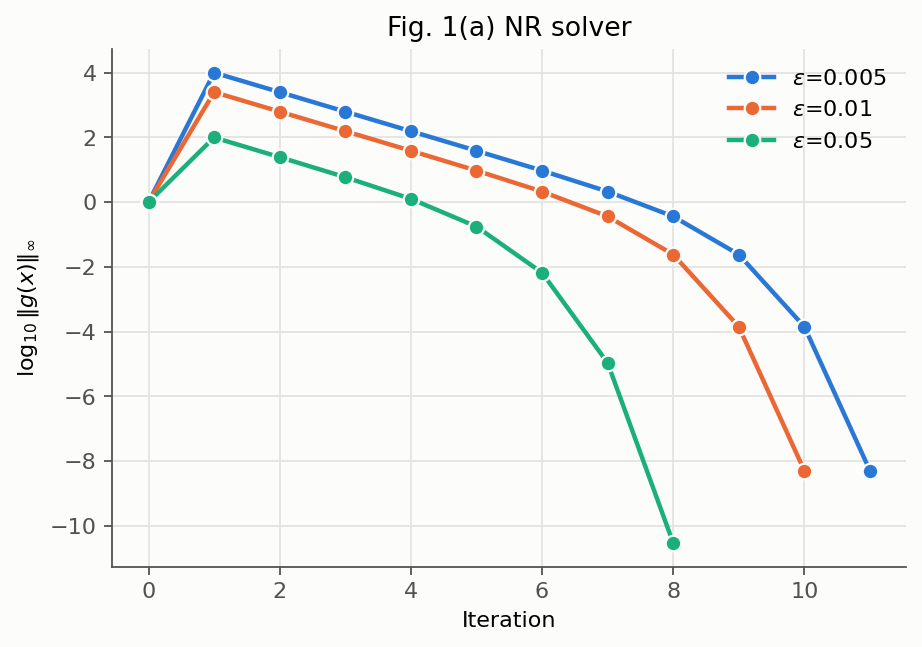
\includegraphics[width=\linewidth]{figures/repo/fig1a_tutorial_nr.png}\caption{NR alone from $(1,1-\epsilon)$}\end{subfigure}\hfill
\begin{subfigure}{0.325\textwidth}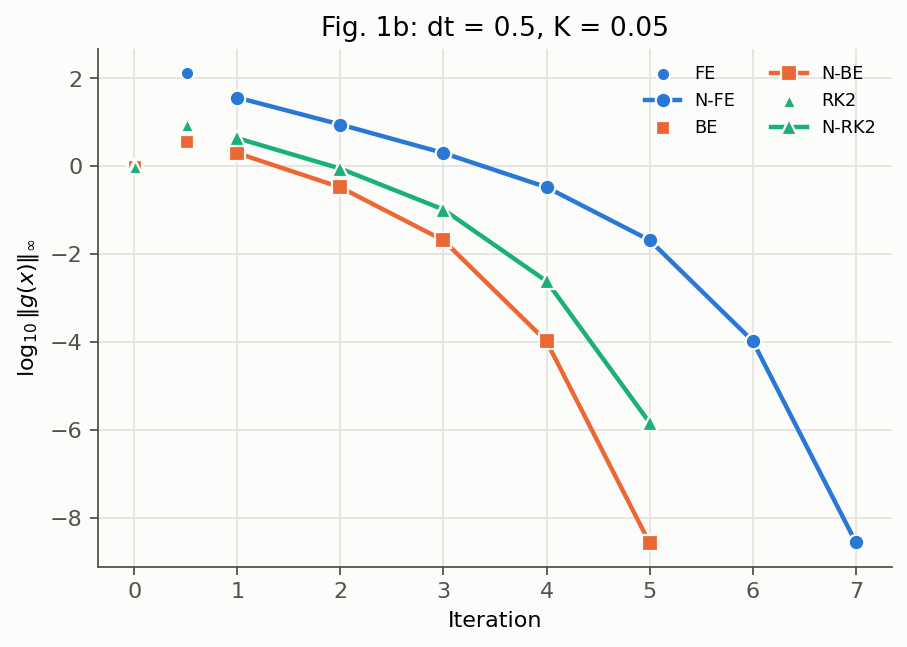
\includegraphics[width=\linewidth]{figures/repo/fig1b_tutorial_hybrid.png}\caption{$\Delta t=0.5$, $K=0.05$}\end{subfigure}\hfill
\begin{subfigure}{0.325\textwidth}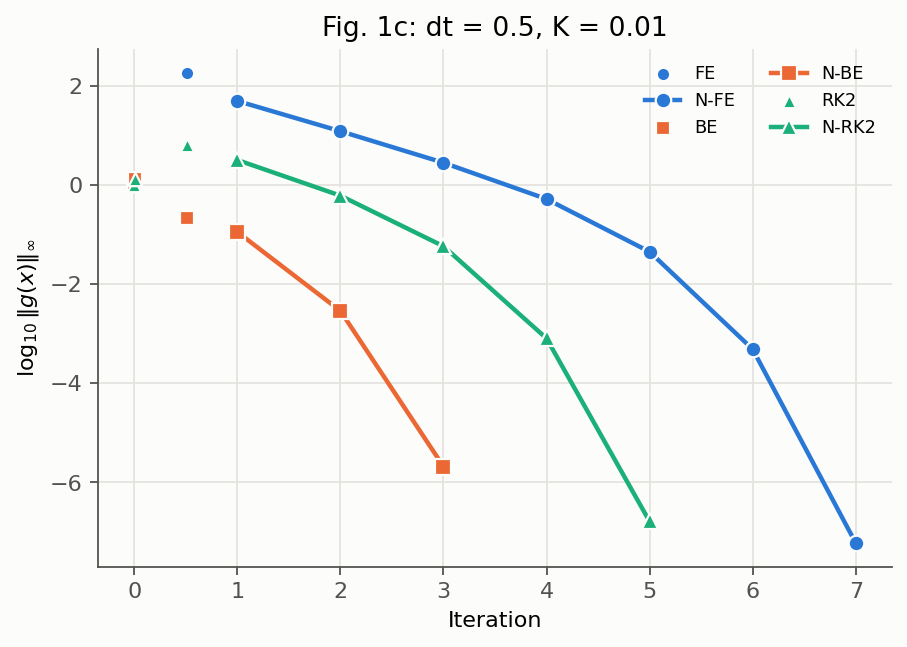
\includegraphics[width=\linewidth]{figures/repo/fig1c_tutorial_hybrid.png}\caption{$\Delta t=0.5$, $K=0.01$}\end{subfigure}\\[4pt]
\begin{subfigure}{0.325\textwidth}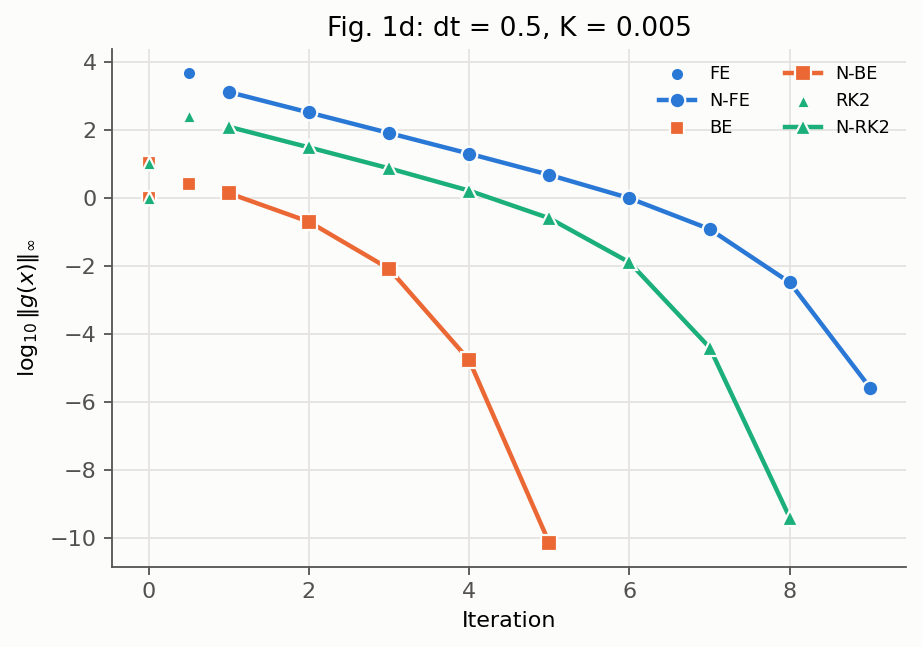
\includegraphics[width=\linewidth]{figures/repo/fig1d_tutorial_hybrid.png}\caption{$\Delta t=0.5$, $K=0.005$}\end{subfigure}\hspace{0.01\textwidth}
\begin{subfigure}{0.325\textwidth}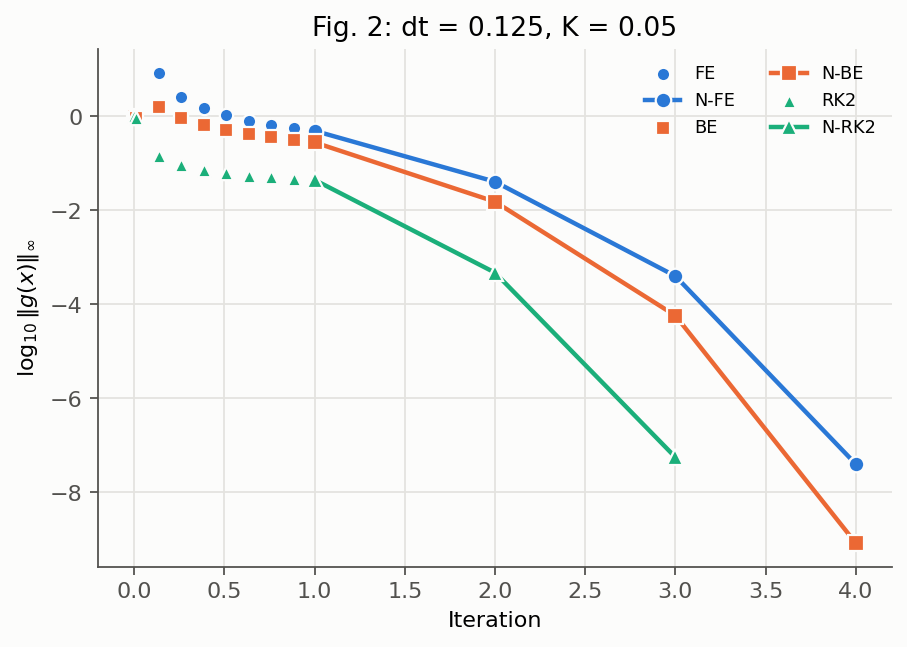
\includegraphics[width=\linewidth]{figures/repo/fig2_tutorial_hybrid.png}\caption{$\Delta t=0.125$, $K=0.05$}\end{subfigure}
\caption{Our versions of the paper's tutorial Figures 1(a)--(d) and 2. Scattered markers are homotopy
points at their time $t\in[0,1]$; connected curves are the NR iterations that follow, iteration $i$ drawn
at $1+i$. BE (orange squares) reaches $10^{-5}$ first in every hybrid panel; in (c) and (d) FE and RK2
converge, but to root $B$.}
\Description{Five semilog plots of mismatch against iteration for the tutorial problem.}
\label{fig:tut-repro}
\end{figure*}

\begin{table*}[!htbp]
\centering
\caption{Table 5 re-run, $K=10^{-4}$: $\ninf{g}$ at each point of the growing-step path and after three NR
iterations.}
\label{tab:t5}
\scriptsize
\setlength{\tabcolsep}{3.5pt}
\begin{tabular}{@{}l l l r r r r r r r r r r@{}}
\toprule
\thead{Case} & \thead{Solver} & & \thead{$t{=}0$} & \thead{0.005} & \thead{0.01} & \thead{0.02} & \thead{0.12} & \thead{0.62} & \thead{1} & \thead{NR 1} & \thead{NR 2} & \thead{NR 3} \\
\midrule
\rows{generated/table5_rows.tex}
\bottomrule
\end{tabular}
\end{table*}

\begin{figure*}[!htbp]
\centering
\begin{subfigure}{0.325\textwidth}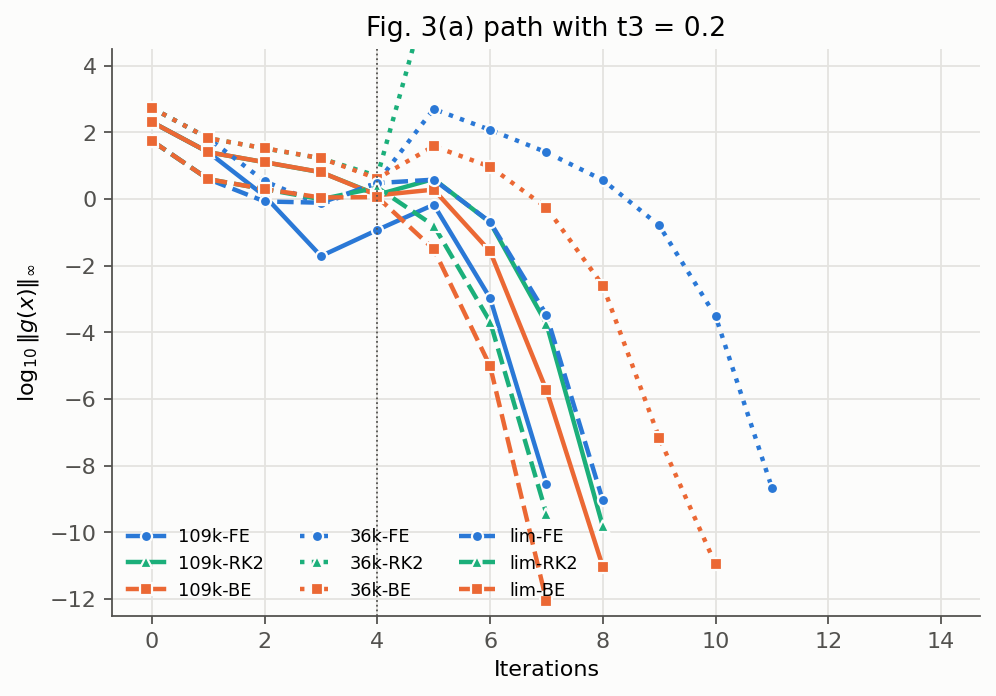
\includegraphics[width=\linewidth]{figures/repo/fig3a_pathway_t3_0.20.png}\caption{$t_3=0.20$}\end{subfigure}\hfill
\begin{subfigure}{0.325\textwidth}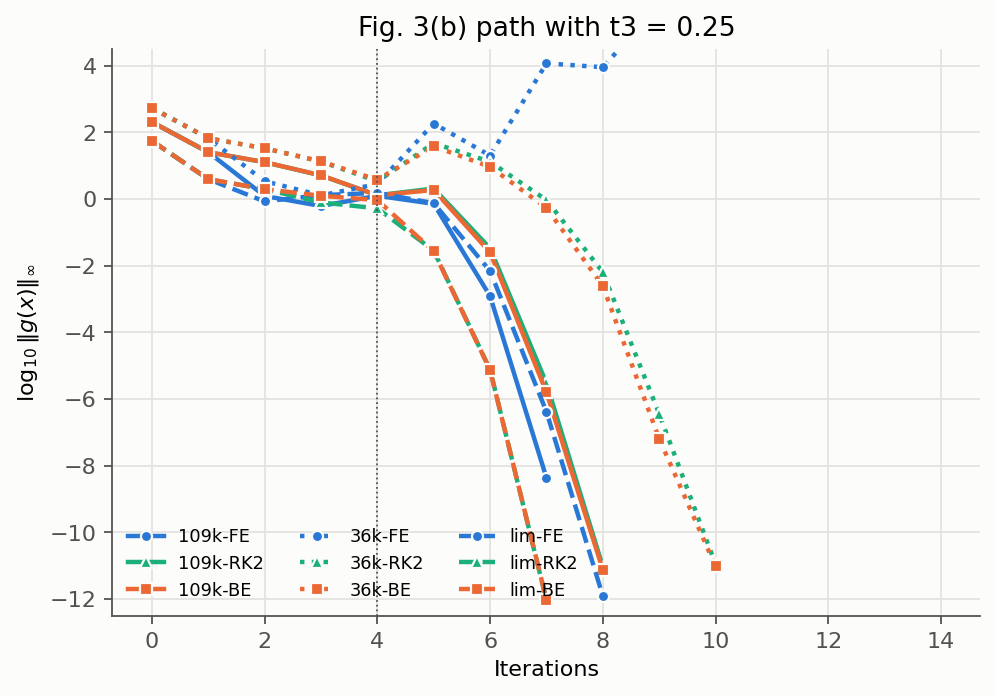
\includegraphics[width=\linewidth]{figures/repo/fig3b_pathway_t3_0.25.png}\caption{$t_3=0.25$}\end{subfigure}\hfill
\begin{subfigure}{0.325\textwidth}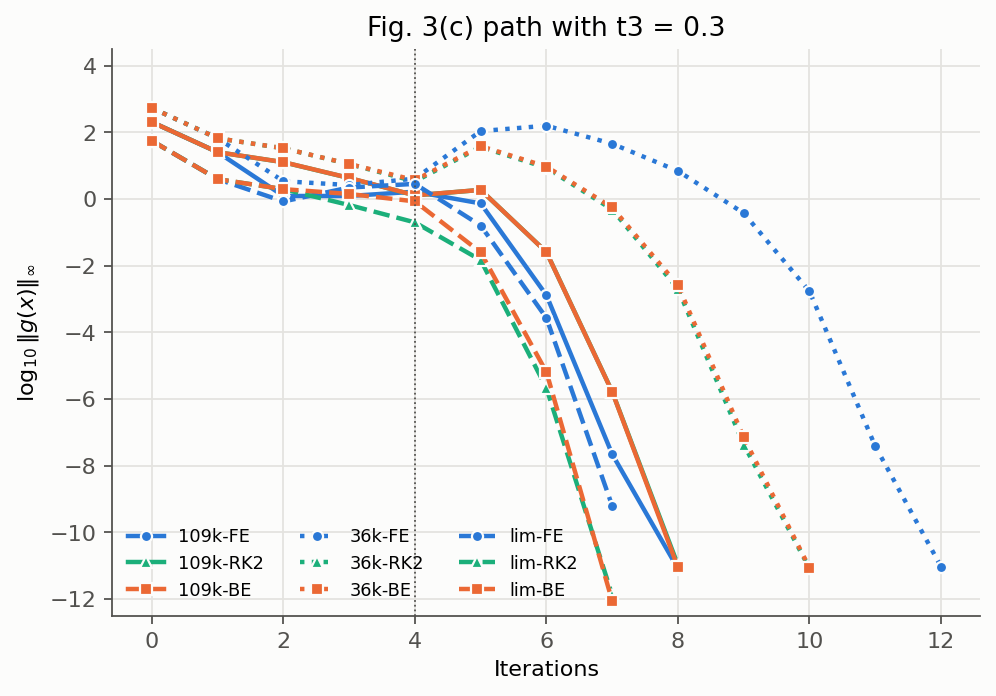
\includegraphics[width=\linewidth]{figures/repo/fig3c_pathway_t3_0.30.png}\caption{$t_3=0.30$}\end{subfigure}
\caption{Figure 3 re-run: $\log_{10}\ninf{g}$ over five homotopy points (0--4) and the NR iterations that
follow, for \code{case109272} (solid), \code{case36964} (dotted) and \code{case2000limit} (dashed).}
\Description{Three line plots of mismatch along five-point paths.}
\label{fig:fig3}
\end{figure*}

\begin{figure*}[!htbp]
\centering
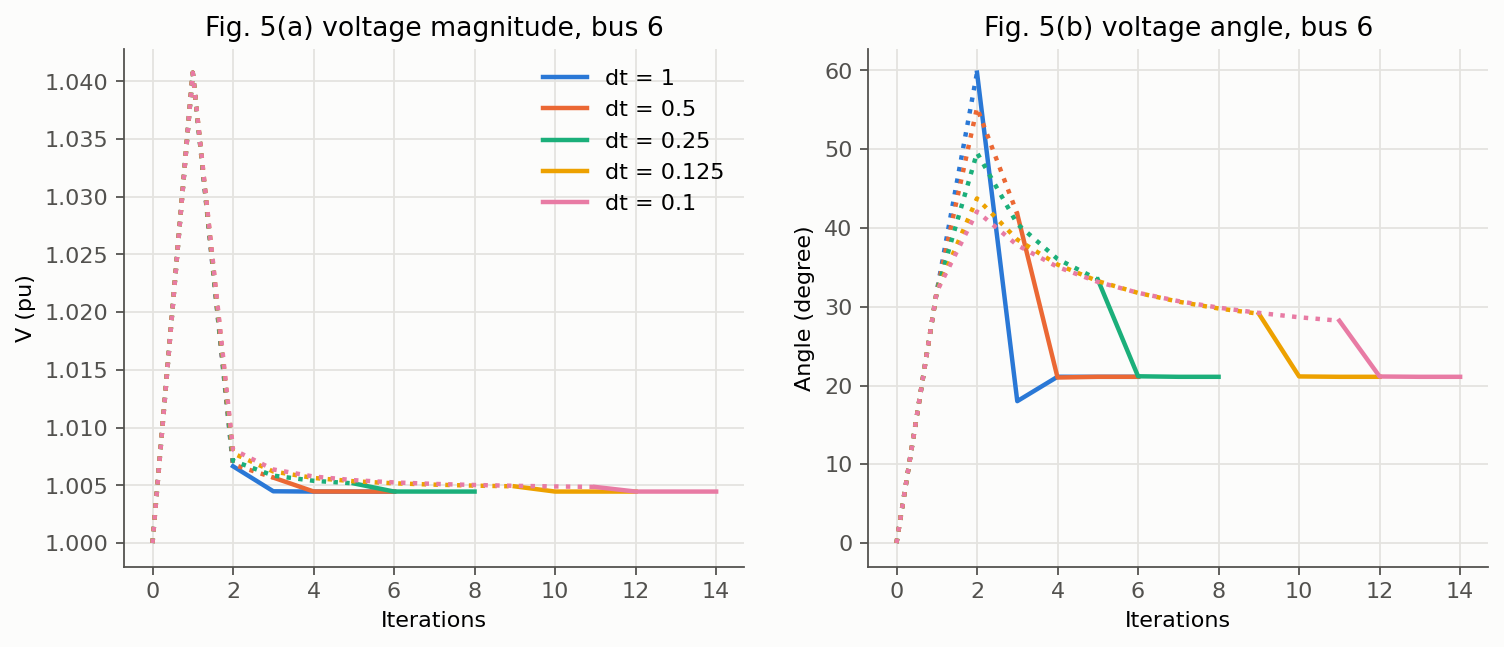
\includegraphics[width=0.85\textwidth]{figures/repo/fig5_timestep_sensitivity.png}
\caption{Figure 5 re-run: voltage magnitude (a) and angle (b) of bus 6 of \code{case109272} for five constant
steps $\Delta t$ after $t_1$; dotted is BE, solid is NR. Every run ends at \SI{1.0045}{pu} and 21.10 degrees.}
\Description{Two line plots of bus 6 voltage and angle for five time steps.}
\label{fig:fig5full}
\end{figure*}

\begin{figure*}[!htbp]
\centering
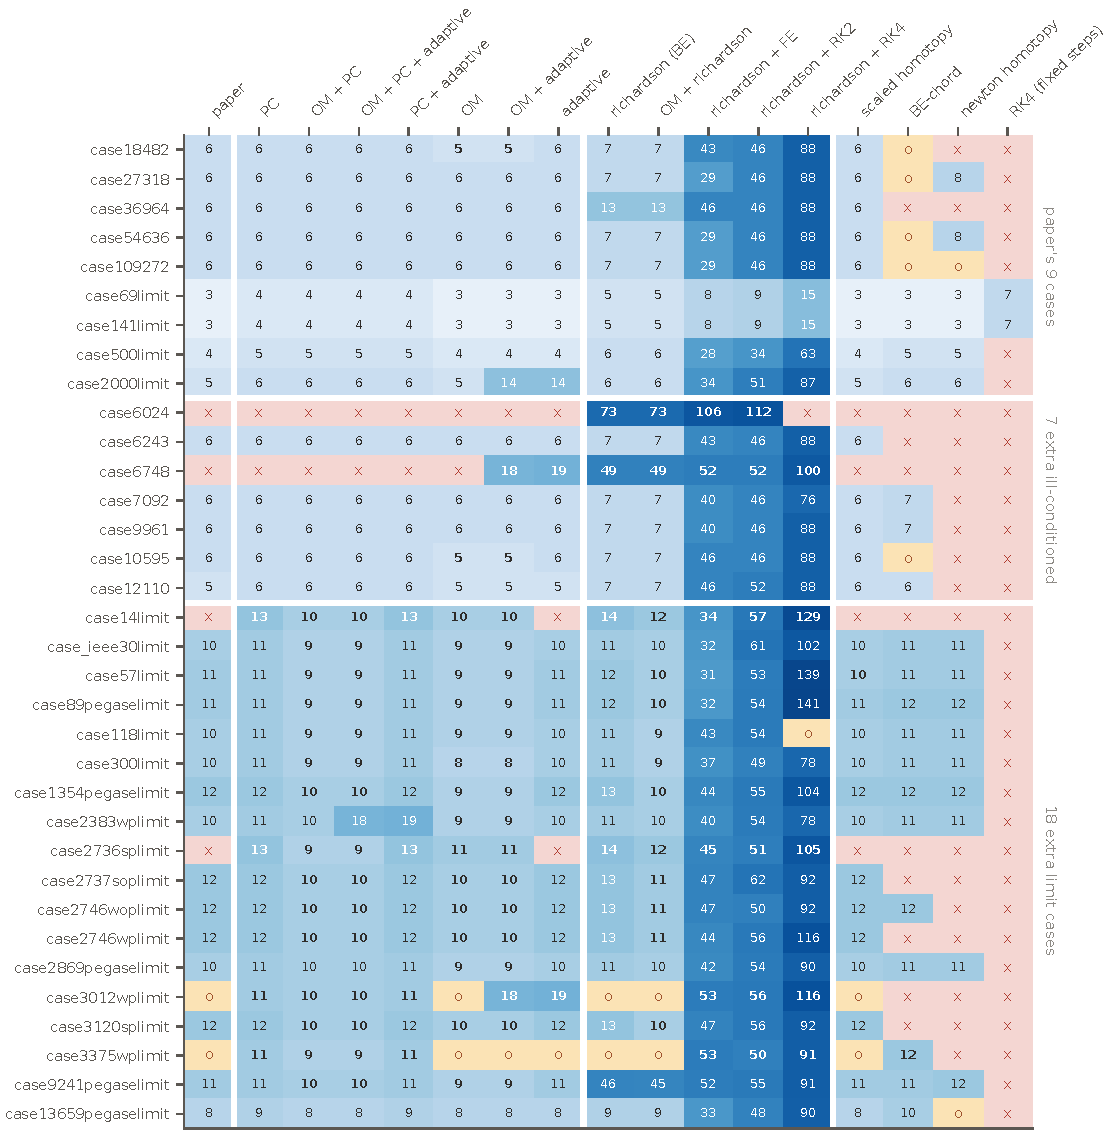
\includegraphics[width=\textwidth]{figures/improve_cases_s1.pdf}
\caption{LU factorizations per system and configuration in S1 (the paper's parameters).
\textcolor{failred}{x}: fails; o: converges to another root. Bold: cheaper than the paper's method or solves a
system it does not.}
\Description{Heat-map table of LU counts per system and configuration.}
\label{fig:cases}
\end{figure*}

\begin{figure*}[!htbp]
\centering
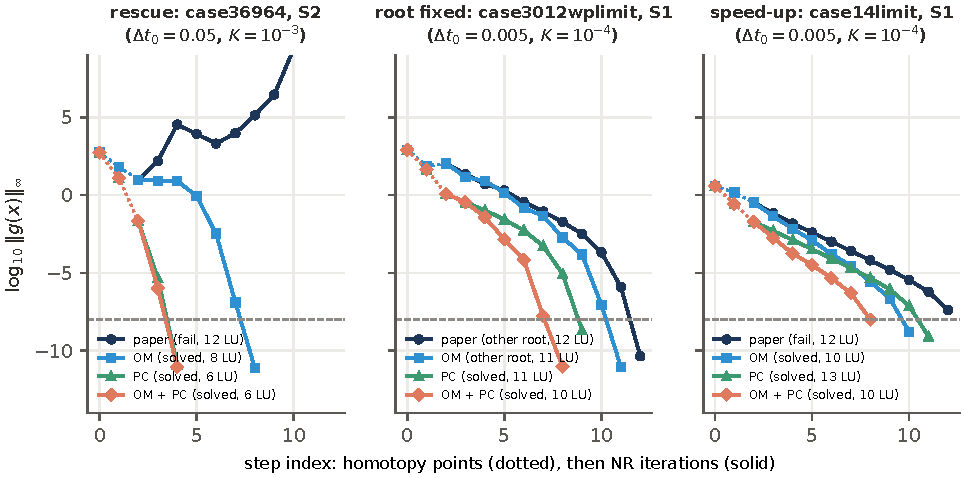
\includegraphics[width=0.92\textwidth]{figures/rescues.pdf}
\caption{Mismatch along the path (dotted) and through NR (solid) for three runs the paper's method does not
solve: a rescue (\code{case36964}, S2), a root fix (\code{case3012wplimit}) and a speed-up
(\code{case14limit}). Dashed: tolerance $10^{-8}$.}
\Description{Three semilog plots of mismatch histories.}
\label{fig:rescues}
\end{figure*}

\begin{figure*}[!htbp]
\centering
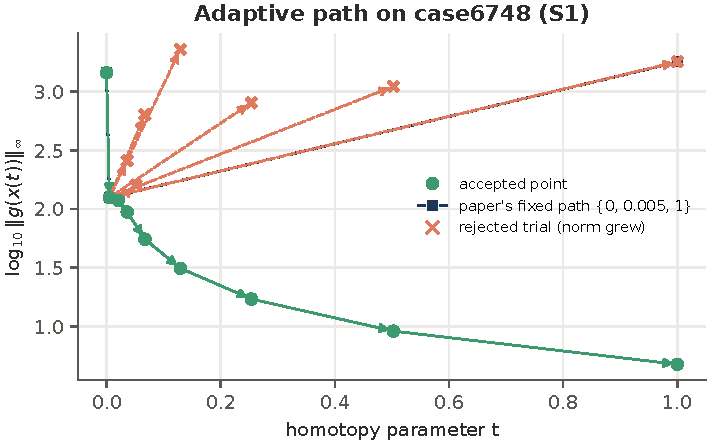
\includegraphics[width=0.55\textwidth]{figures/adaptive_path.pdf}
\caption{Every step the adaptive rule (with the multiplier) tries on \code{case6748}, S1. Green: accepted;
orange: rejected trials, which still cost an LU. Navy squares: the paper's fixed path.}
\Description{Plot of accepted and rejected adaptive steps.}
\label{fig:adaptive}
\end{figure*}

\FloatBarrier
\section{Member Contributions}\label{app:contrib}
All five members contributed equally. Every member owns one part of the core code, one part of
the paper's results, one modification and one numerical study from the proposal, the report figures and
tables built from that work, and the tests for their own code (\cref{tab:contrib}). The details follow by
roll number; the full account is in \code{CONTRIBUTIONS.md} in the repository~\cite{ourrepo}.

\begin{table*}[!htbp]
\centering
\caption{Contributions of each group member, by roll number.}
\label{tab:contrib}
\footnotesize
\begin{tabularx}{\textwidth}{@{}>{\raggedright\arraybackslash}p{2.6cm} >{\raggedright\arraybackslash}X >{\raggedright\arraybackslash}X >{\raggedright\arraybackslash}X >{\raggedright\arraybackslash}X@{}}
\toprule
\thead{Roll, member} & \thead{Core code} & \thead{Paper results} & \thead{Modifications and studies} & \thead{Report and tests} \\
\midrule
2105039\newline Mohiuddin Sizan & Table output in CSV and Markdown, paper values side by side, timing benchmark & Tables 2--6, Figure 3 & FE, RK2, RK4 and BE-chord step rules; golden-section tuning of $\delta$ & Tables 2--5 in \LaTeX, fidelity plot, tuning figure; Table~4 regression test, explicit first step, golden section \\
2105040\newline Sadman bin Tareq & Sparse LU with the LU counter, result types, figure style & Section 4.4, Figure 5 & Richardson step control, scaled homotopy; Gauss elimination and LU from scratch; command-line tool & Jacobian sparsity, Section 4.4 grid, Figure 5 cost, Richardson paths; tests of Gauss/LU, pivoting, Richardson, scaled homotopy, CLI \\
2105057\newline Mosharaf Hossain Apurbo & Fixed-point homotopy, FE/BE/RK2 integrators, path schedules, hybrid method & Figures 1, 2, 4, Section 4.2.1 & \code{solve()} with switches, Newton corrector, adaptive steps; spectrum of the Jacobian & Tutorial geometry, first step, adaptive path, spectrum figures; tests of path, first step, tutorial, switch-off identity, corrector, eigenvalues \\
2105058\newline Elias Hasbi & NR, FDXB (XB), reconstruction of GSH-NR & Tables 7, 8 & Optimal multiplier, Newton homotopy; NR and FDXB with our own LU & Timing, cost against robustness, per-case map, rescue histories; tests of NR/FDXB counts, multiplier, own-LU iterates, Newton homotopy \\
2105060\newline Jonayed Mohiuddin Shanto & Public GitHub repository; power flow model ($g$, $J$, case reader) and the solver interface; test-system download, experiment runner & Flat-start check and base-MVA finding, root check of Table 7, audit of the paper & Wider test bed of 34 systems, solution (root) check, the comparison study of all modifications; feasibility maps & Test-systems table and figure, audit table, feasibility figure, study summary figure and table; Jacobian test \\
\bottomrule
\end{tabularx}
\end{table*}

\paragraph{2105039, Mohiuddin Sizan}
Wrote the table output that prints every reproduced value next to the paper's, and the median-of-runs
timing benchmark. Reproduced the paper's Tables 2--6 and Figure 3, including the paper's one failure on
\code{case36964}. Added the FE, RK2, RK4 and BE-chord step rules and showed, with Sadman's Richardson
control, that BE stays the cheapest integrator under error control (10.6 LUs in S1 against 37, 48 and 87).
Built the golden-section tuning of $\delta$ and the test of fixed and spectral rules (\cref{tab:tuning}).

\paragraph{2105040, Sadman bin Tareq}
Wrote the sparse LU wrapper whose counter is the cost measure of the whole project, the result types and
the figure style. Reproduced Section 4.4 and Figure 5. Built Richardson step control, the only change that
solves some systems nothing else solves, and the scaled homotopy; wrote Gauss elimination and LU with
partial pivoting from scratch, and the command-line tool \code{python -m improvements}.

\paragraph{2105057, Mosharaf Hossain Apurbo}
Implemented the core of the paper: the fixed-point homotopy, its three integrators and the hybrid method,
and showed that the BE first step equals the paper's linearised static homotopy. Reproduced Figures 1, 2, 4
and Section 4.2.1. Built the \code{solve()} framework that switches every modification on and off, the
Newton corrector (152 runs solved, none lost) and adaptive steps, and the spectral study of the flat-start
Jacobian.

\paragraph{2105058, Elias Hasbi}
Wrote NR, FDXB and the reconstruction of GSH-NR, and found the paper's way of counting FDXB iterations.
Reproduced Tables 7 and 8. Built the optimal multiplier, which with Apurbo's corrector gives the
recommended configuration (152 runs, 7\% fewer LUs), the Newton homotopy, and NR and FDXB running on our
own LU (\cref{tab:ownlu}).

\paragraph{2105060, Jonayed Mohiuddin Shanto}
Set up and maintains the project's public GitHub repository~\cite{ourrepo}, where the code of all five
members comes together. Built the power flow model that every other part runs on: the case reader, the
equations $g(x)$ and the Jacobian $J(x)$, and the \code{g}/\code{jacobian} interface against which every
solver, integrator and modification of the team is written, so that the same code runs on the $2\times2$
tutorial and on the 109{,}272-bus grid. Wrote the download of the test systems and the runner of all 15
experiments, which reproduces the whole project with one command. Found the base-MVA inconsistency of the
two small limit cases, checked every Table~7 run against the reference solution, and compiled the audit of
the paper (\cref{tab:audit}). Widened the test bed from 9 to 34 systems and wrote the solution (root) check
behind the project's main finding---14 of the paper's 141 converged runs reach another root. That check is
used throughout the project: in Table~7, the comparison study, the feasibility maps, the tuning of $\delta$
and the command-line tool. Wrote the comparison study in which the work of all members meets: it runs
every member's modification, alone and combined, on 34 systems under five settings (2{,}890 runs), and
separates rescues, root fixes and speed-ups (\cref{tab:improve}). Built the feasibility maps of the
$(K,\Delta t_0)$ plane, which explain the paper's unexplained failure at $\Delta t_0=0.1$.

\end{document}
